%%% The main file. It contains definitions of basic parameters and includes all other parts.

%% Settings for single-side (simplex) printing
% Margins: left 40mm, right 25mm, top and bottom 25mm
% (but beware, LaTeX adds 1in implicitly)
\documentclass[12pt,a4paper,rgb,hyperref,rgb,hyperref,table,xcdraw]{report}
\setlength\textwidth{145mm}
\setlength\textheight{247mm}
\setlength\oddsidemargin{15mm}
\setlength\evensidemargin{15mm}
\setlength\topmargin{0mm}
\setlength\headsep{0mm}
\setlength\headheight{0mm}
% \openright makes the following text appear on a right-hand page
\let\openright=\clearpage

%% Settings for two-sided (duplex) printing
% \documentclass[12pt,a4paper,twoside,openright]{report}
% \setlength\textwidth{145mm}
% \setlength\textheight{247mm}
% \setlength\oddsidemargin{14.2mm}
% \setlength\evensidemargin{0mm}
% \setlength\topmargin{0mm}
% \setlength\headsep{0mm}
% \setlength\headheight{0mm}
% \let\openright=\cleardoublepage

%% Generate PDF/A-2u
\usepackage[a-2u]{pdfx}

%% Character encoding: usually latin2, cp1250 or utf8:
\usepackage[utf8]{inputenc}
%% Prefer Latin Modern fonts
\usepackage{lmodern}
\usepackage{hyperref}

\usepackage{textcomp}
\DeclareUnicodeCharacter{00B4}{}


%% Further useful packages (included in most LaTeX distributions)
\usepackage{todonotes}
\usepackage{nameref}
\usepackage{amsmath}        % extensions for typesetting of math
\usepackage{amsfonts}       % math fonts
\usepackage{amsthm}         % theorems, definitions, etc.
\usepackage{bbding}         % various symbols (squares, asterisks, scissors, ...)
\usepackage{bm}             % boldface symbols (\bm)
\usepackage{graphicx}       % embedding of pictures
\usepackage{fancyvrb}       % improved verbatim environment
\usepackage{natbib}  
\usepackage{multirow}
\usepackage{float}
\usepackage{breakcites}
\setcitestyle{authordate}
      % citation style AUTHOR (YEAR), or AUTHOR [NUMBER]
\usepackage[nottoc]{tocbibind} % makes sure that bibliography and the lists
			    % of figures/tables are included in the table
			    % of contents
\usepackage{dcolumn}        % improved alignment of table columns
\usepackage{booktabs}       % improved horizontal lines in tables
\usepackage{paralist}       % improved enumerate and itemize
\usepackage[automake,toc]{glossaries} %for list of abbreviations
\usepackage{threeparttable}
\makeglossaries
\setacronymstyle{long-short}
\loadglsentries{defns}
%\usepackage[rgb,hyperref,rgb,hyperref,table,xcdraw]{xcolor}
%%% Basic information on the thesis


% Thesis title in English (exactly as in the formal assignment)
\def\ThesisTitle{Czech NLP with Contextualized Embeddings}

% Author of the thesis
\def\ThesisAuthor{Bc. Petra Vysušilová}

% Year when the thesis is submitted
\def\YearSubmitted{2021}

% Name of the department or institute, where the work was officially assigned
% (according to the Organizational Structure of MFF UK in English,
% or a full name of a department outside MFF)
\def\Department{Institute of Formal and Applied Linguistics}

% Is it a department (katedra), or an institute (ústav)?
\def\DeptType{Institute} 

% Thesis supervisor: name, surname and titles
\def\Supervisor{RNDr. Milan Straka, Ph.D.}

% Supervisor's department (again according to Organizational structure of MFF)
\def\SupervisorsDepartment{Institute of Formal and Applied Linguistics}

% Study programme and specialization
\def\StudyProgramme{Computer science}
\def\StudyBranch{Artificial intelligence}

% An optional dedication: you can thank whomever you wish (your supervisor,
% consultant, a person who lent the software, etc.)
\def\Dedication{%
Firstly, I would like to express my gratitude to my supervisor, Milan Straka, for answering even the dumbest questions with patience and kindness, helping me to debug tricky errors, but also the obvious ones, and always being cheerful and full of enthusiasm. I learned so much during the work on this thesis. \\
This thesis could not be possible without my loving husband and his continuous support. I would also like to thank my s[o/u]n, who didn't let me programming all day without interruption and go crazy. \\
I could never start studying without my mom and grandma, who raised me and gave me the best. \\
Last but not least, Thank God, who created such a beautiful world.\\ \\
P.S.: My husband wants me to write here that he is amazing (and he truly is).
}

% Abstract (recommended length around 80-200 words; this is not a copy of your thesis assignment!)
\def\Abstract{
%Recently, several methods for unsupervised pre-training of contextualized word embeddings have been proposed, most importantly the BERT model (Devlin et al., 2018). Such contextualized representations have been extremely useful as additional features in many NLP tasks like morphological or syntactic analysis, entity recognition or text classification.

%Most of the evaluation have been carried out on English. However, several of the released models have been pre-trained on many languages including Czech, like multilingual BERT or XLM-RoBERTa (Conneau et al, 2019). Therefore, the goal of this thesis is to perform experiments quantifying improvements of employing pre-trained contextualized representation in Czech natural language processing.
}

% 3 to 5 keywords (recommended), each enclosed in curly braces
\def\Keywords{%
{Natural Language Processing} {BERT} {Bidirectional Encoder Representations from Transformers} 
}

%% The hyperref package for clickable links in PDF and also for storing
%% metadata to PDF (including the table of contents).
%% Most settings are pre-set by the pdfx package.
\hypersetup{unicode}
\hypersetup{breaklinks=true}

% Definitions of macros (see description inside)
%%% This file contains definitions of various useful macros and environments %%%
%%% Please add more macros here instead of cluttering other files with them. %%%

%%% Minor tweaks of style

% These macros employ a little dirty trick to convince LaTeX to typeset
% chapter headings sanely, without lots of empty space above them.
% Feel free to ignore.
\makeatletter
\def\@makechapterhead#1{
  {\parindent \z@ \raggedright \normalfont
   \Huge\bfseries \thechapter. #1
   \par\nobreak
   \vskip 20\p@
}}
\def\@makeschapterhead#1{
  {\parindent \z@ \raggedright \normalfont
   \Huge\bfseries #1
   \par\nobreak
   \vskip 20\p@
}}
\makeatother

% This macro defines a chapter, which is not numbered, but is included
% in the table of contents.
\def\chapwithtoc#1{
\chapter*{#1}
\addcontentsline{toc}{chapter}{#1}
}

% Draw black "slugs" whenever a line overflows, so that we can spot it easily.
\overfullrule=1mm

%%% Macros for definitions, theorems, claims, examples, ... (requires amsthm package)

\theoremstyle{plain}
\newtheorem{thm}{Theorem}
\newtheorem{lemma}[thm]{Lemma}
\newtheorem{claim}[thm]{Claim}

\theoremstyle{plain}
\newtheorem{defn}{Definition}

\theoremstyle{remark}
\newtheorem*{cor}{Corollary}
\newtheorem*{rem}{Remark}
\newtheorem*{example}{Example}

%%% An environment for proofs

%%% FIXME %%% \newenvironment{proof}{
%%% FIXME %%%   \par\medskip\noindent
%%% FIXME %%%   \textit{Proof}.
%%% FIXME %%% }{
%%% FIXME %%% \newline
%%% FIXME %%% \rightline{$\square$}  % or \SquareCastShadowBottomRight from bbding package
%%% FIXME %%% }

%%% An environment for typesetting of program code and input/output
%%% of programs. (Requires the fancyvrb package -- fancy verbatim.)

\DefineVerbatimEnvironment{code}{Verbatim}{fontsize=\small, frame=single}

%%% The field of all real and natural numbers
\newcommand{\R}{\mathbb{R}}
\newcommand{\N}{\mathbb{N}}

%%% Useful operators for statistics and probability
\DeclareMathOperator{\pr}{\textsf{P}}
\DeclareMathOperator{\E}{\textsf{E}\,}
\DeclareMathOperator{\var}{\textrm{var}}
\DeclareMathOperator{\sd}{\textrm{sd}}

%%% Transposition of a vector/matrix
\newcommand{\T}[1]{#1^\top}

%%% Various math goodies
\newcommand{\goto}{\rightarrow}
\newcommand{\gotop}{\stackrel{P}{\longrightarrow}}
\newcommand{\maon}[1]{o(n^{#1})}
\newcommand{\abs}[1]{\left|{#1}\right|}
\newcommand{\dint}{\int_0^\tau\!\!\int_0^\tau}
\newcommand{\isqr}[1]{\frac{1}{\sqrt{#1}}}

%%% Various table goodies
\newcommand{\pulrad}[1]{\raisebox{1.5ex}[0pt]{#1}}
\newcommand{\mc}[1]{\multicolumn{1}{c}{#1}}


% Title page and various mandatory informational pages
\begin{document}
%%% Title page of the thesis and other mandatory pages

%%% Title page of the thesis

\pagestyle{empty}
\hypersetup{pageanchor=false}
\begin{center}

\centerline{\mbox{
\includegraphics[width=166mm]{../img/logo-en.pdf}}}

\vspace{-8mm}
\vfill

{\bf\Large MASTER THESIS}

\vfill

{\LARGE\ThesisAuthor}

\vspace{15mm}

{\LARGE\bfseries\ThesisTitle}

\vfill

\Department

\vfill

\begin{tabular}{rl}

Supervisor of the master thesis: & \Supervisor \\
\noalign{\vspace{2mm}}
Study programme: & \StudyProgramme \\
\noalign{\vspace{2mm}}
Study branch: & \StudyBranch \\
\end{tabular}

\vfill

% Zde doplňte rok
Prague \YearSubmitted

\end{center}

\newpage

%%% Here should be a bound sheet included -- a signed copy of the "master
%%% thesis assignment". This assignment is NOT a part of the electronic
%%% version of the thesis. DO NOT SCAN.

%%% A page with a solemn declaration to the master thesis

\openright
\hypersetup{pageanchor=true}
\pagestyle{plain}
\pagenumbering{roman}
\vglue 0pt plus 1fill

\noindent
I declare that I carried out this master thesis independently, and only with the cited
sources, literature and other professional sources.

\medskip\noindent
I understand that my work relates to the rights and obligations under the Act No.~121/2000 Sb.,
the Copyright Act, as amended, in particular the fact that the Charles
University has the right to conclude a license agreement on the use of this
work as a school work pursuant to Section 60 subsection 1 of the Copyright Act.

\vspace{10mm}

\hbox{\hbox to 0.5\hsize{%
In ........ date ............	% FIXME!
\hss}\hbox to 0.5\hsize{%
signature of the author
\hss}}

\vspace{20mm}
\newpage

%%% Dedication

\openright

\noindent
\Dedication

\newpage

%%% Mandatory information page of the thesis

\openright

\vbox to 0.5\vsize{
\setlength\parindent{0mm}
\setlength\parskip{5mm}

Title:
\ThesisTitle

Author:
\ThesisAuthor

\DeptType:
\Department

Supervisor:
\Supervisor, \SupervisorsDepartment

Abstract:
\Abstract

Keywords:
\Keywords

\vss}

\newpage

\openright
\pagestyle{plain}
\pagenumbering{arabic}
\setcounter{page}{1}


%%% A page with automatically generated table of contents of the master thesis

\tableofcontents


%%% Abbreviations used in the thesis, if any, including their explanation
%%% In mathematical theses, it could be better to move the list of abbreviations to the beginning of the thesis.
%\chapwithtoc{List of Abbreviations}
\printglossary[title=List of Abbreviations]

%%% Each chapter is kept in a separate file
\chapter*{Introduction}
\addcontentsline{toc}{chapter}{Introduction}


This work aim to improve some natural language processing (NLP) tasks for Czech \todo{seznam zkratek} with the use of recently published artificial intelligence (AI) state-of-the-art techniques. In Deep Learning book \cite, NLP is
defined as "...the use of human languages, such as English or French, by a computer." \cite[]{Goodfellow-et-al-2016}. NLP offers a variety of problems to solve from oral--written language conversion, machine translation, syntax analysis used for automatic grammar correction as well as it serve as a base for further linguistic processing. Semantic analysis includes in addition to already mentioned machine translation tasks like sentiment analysis, natural language text generation or recognition
of homonymy or polysemy of given words. It could solve sophisticated assignments as answering questions about the input text document.

\cite{BERT_ORIG}
\section*{Tasks definition}
\todo{obrazky k taskum s priklady}
This work aims to apply the most successful NLP methods of recent years to Czech NLP task - namely tagging, lemmatization and sentiment analysis. Tagging and lemmatization represents syntax analysis, in contrast with sentiment analysis which represents semantic type of tasks. \todo{dát priklady jinych tasku}
The practical part of this work is focused on these tasks:
\begin{itemize}
\item POS tagging \\
\textit{input}: a word \\
\textit{output}: part-of-speech tags -- as noun, pronoun, punctuation mark etc.
\item lemmatization \\
\textit{input:} a word \\
\textit{output:} lemma -- a base form of a given words, meaning for example nominative of singular for nouns or infinitive for verbs. 
\item sentiment analysis \\
\textit{input:} a sentence or a sequence of sentences \\
\textit{output:} prevailing sentiment of the input from categories: neutral, positive, negative.
\todo{doplnit diskuzi o ruzných možnostech definice}
\end{itemize}.

These tasks were chosen to show how pre-trained multilingual language models can help with different types of NLP tasks in one of trained langugages. 

\section*{Text structure}
Theoretical background in NLP and used AI methods and related work is provided in the \hyperref[chap:theandme]{following chapter}.

Implementation documentation in chapter \ref{chap:impl} is followed by discussion about used methods and experiment results in chapter \ref{chap:diss} Result models are accessible to user exploration as described in chapter \ref{chap:userdoc} and text is closed by \hyperref[chap:concl]{conclusion} with future work proposals.



\chapter{Title of the first chapter}

An~example citation: \cite{Andel07}

\section{Title of the first subchapter of the first chapter}

\section{Title of the second subchapter of the first chapter}

\chapter{Experiments}
This chapter describes all experiments and their results. First part is dedicated to presentation of different experiement hyperparameters, which are in many cases common to all tasks, followed by the analysis of each task -- definition, related work, datasets, a description of according model and results.
\section{A description of training hyperparameters}
\subsection{General experiment setup (EXPE)}
Training is performed in one of following settings:
\begin{itemize}
\item \textbf{base}: Baseline implementation (described separately for each task, typically without using advanced language models).
\item \textbf{ls}: This setup uses same setting as baseline implementation but with label smoothing.
\item \textbf{embed}: BERT-like language model is used only to generate static embeddings in advanced. These embeddings are not further trained.
\item \textbf{fine}: Fine-tuning consist in dividing the training time into two parts. Firstly, rest of the model is trained with BERT layers frozen (not trained), so it is same as the \textit{embed} settings. In the second part, the whole model is trained together.
\item \textbf{simple}: Model architecture is reduced to bert layers with a simple classification head. This is basic setting for all sentiment analysis experiments.\footnote{For tagging and lemmatization, all previously mentioned EXPE setups are performed with more sophisticated classification head than in \textit{simple} version.} 
\item \textbf{full}: This options means training the whole model from the beginning (in contrast to \textit{fine} option), but the classification head is not simplified (in contrast \textit{simple} option).
\end{itemize}
%TODO zmenit u sentimentu mít všude simple nebo full a jinej sloupec na data?
\subsection{Training data}
Tagging and lemmatization tasks use same set of data for every experiments, co there is no need for separate description. Sentiment analysis task, however, uses three possible options for a selection of training data:
\begin{itemize}
\item \textbf{mall|facebook|csfd}: Model is trained and evaluated on the (sub)set of czech datasets.
\item \textbf{zero}: Model is trained on english sentiment analysis dataset, but evaluated on czech data.
\item \textbf{eng}: Model is trained on the combination of czech and english training data (and evaluated again on the czech data). %TODO pridat jeste jednotlive ceske datasety
\end{itemize}
\subsection{Learning rate scheduling type (LRTYPE)}
Most experiments are expected to perform better with some kind of learning rate scheduling. This work implements three types of learning rate scheduling:
\begin{itemize}
\item \textbf{simple} \textit{Simple} option indicates no more complex learning rate scheduling than setting in advance different learning rates for different epochs.
\item \textbf{isrd} %TODO citovat 
\textit{isrd} means inverse square root learning rate decay defined by formula: $1/\sqrt{max(n,k)}$ where $k$ is the number of so-called \textit{warmup steps} and $n$ is the current iteration. This leads to constant learning rate for first $k$ steps and decayed learning rate in rest of iterations.
\item \textbf{cos}: Another learning rate scheduling used in this work is \textit{cosine decay} %TODO citovat
which applies following formula: $$lr=lr_{min}^{i} + \frac{1}{2}(lr_{max}^{i} - lr_{min}^{i})(1+cos(\frac{T_{curr}}{T_i}\pi)),$$ where $lr_{min}^{i}$ and $lr_{min}^{i}$ is the range of the learning rate, $T_i$ is the number of epochs after which the learning rate is restarted, i.e. increased to the $lr_{max}^{i}$ value and $T_{curr}$ is the current epoch number.
\end{itemize}

\subsection{Model layers selected for embeddings (LAYERS)}
As discussed in the previous chapter, is unclear how to extract best embeddings from the language model, especially which layers to take into account. By selecting the most promising ways, following two hyperparameters are used in this work:
\begin{itemize}
\item \textbf{four}: Last four of the model are averaged to obtain final embeddings.
\item \textbf{att}: This setting performs weighted sum of all model layers and the weights are trained during training together with the rest of the model.
\end{itemize}
Experiments are also performed with different learning rates (LR), batch size (BATCH) and a number of epochs (EPOCH). 
Technical details needed for running scripts can be found in chapter \ref{chap:impl}.
\newpage
\section{Lemmatization and part-of-speech tagging}
\label{chap:tag}
Lemmatization and \acrshort{pos} tagging tasks are categorized as morphological analysis, share the same architecture and trained network and they will be described together in this section.
\subsection{Task Definition}

\paragraph{\textbf{POS tagging}} \mbox{}\\
\textit{input}: a sequence of  words \\
\textit{output}: tag (for each word), which contains not only part-of-speech (e.g. noun, pronoun, punctuation mark) but also other morphological analysis (case, tense, etc) corresponding to 15-places morphological tagging system by \cite{Hajic2004}. Description of each position can be found in table \ref{Tab:tagset}.

\paragraph{\textbf{Lemmatization}} \mbox{}\\
\textit{input:} a sequence of words \\
\textit{output:} lemma (for each word) -- a base form of a given words, for example nominative of singular for nouns or infinitive for verbs. In this work, lemmatization is treated as a classification problem with classes coresponding to generating rules which transform an input word into target lemma. For example of such rules see figure \ref{fig:lemma_rules}. \\

\begin{table}[!ht]
\centering
\begin{tabular}{ |c|c|c| } 
 \hline
 Position & Name & Description \\ 
 \hline \hline
 1 & POS & Part of speech \\ \hline
 2 & SubPOS & Detailed part of speech \\ \hline
  3 & Gender & Gender \\ \hline
4 & Number & Number \\\hline
  5 & Case & Case \\ \hline
 6 & PossGender & Possessor's gender \\\hline
  7 & PossNumber & Possessor's number \\ \hline
8 & Person & Person \\\hline
  9 & Tense & Tense \\ \hline
 10 & Grade & Degree of comparison\\\hline
  11 & Negation & Negation \\ \hline
 12 & Voice & Voice \\\hline
 13 & Reserve1 & Reserve \\ \hline
14 & Reserve2 & Reserve \\\hline
  15 & Var & Variant, style \\ 
 \hline
\end{tabular}
\caption[Czech morphological tags]{Czech morphology developement is dated from 1989 \citep{Hajic2004} 
and in description of words uses 15-places morphological tags as described in this table taken from \url{https://ufal.mff.cuni.cz/pdt2.0/doc/manuals/en/m-layer/html/ch02s02s01.html}. For more detailed  description or for exploration of predictions given by this work is recommended to use website of Institute of Theoretical and Computational linguistics: \url{http://utkl.ff.cuni.cz/~skoumal/morfo/?pos=11\&val=1}, although they use slightly different set with additional 16 position. }
\label{Tab:tagset}
\end{table}

\paragraph{Metrics} Accuracy is used for the evaluation and is reported separately for several options -- only tags/lemmas, accuracy of joint classification of tags and lemmas, and  also all three variants with an usage of a morphological dictionary (this option is described in more detail in \ref{sub:dataset}).

\begin{figure}[!ht]
\centering
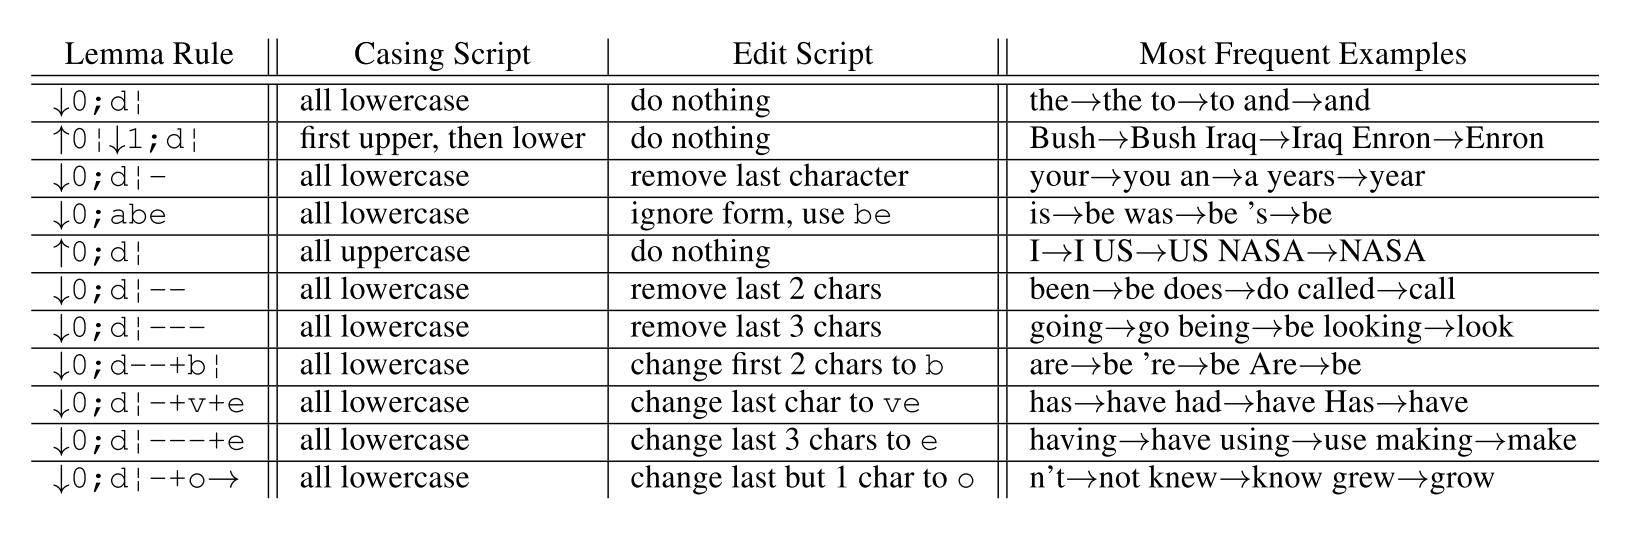
\includegraphics[width=1\textwidth]{../img/lemma_rules}
\protect\caption[The most common lemma generating rules in English EWT corpus]{
Table 1 from \citep{Straka2019b} presents 10 most common lemma generating rules in English EWT corpus. Each rule has two parts -- a casing script for transforming uppercase and lowercase letters, and an edit script. The edit script can transform prefix, suffix, or also a root of the word. It uses the Wagner–Fischer algorithm \citep{Wagner}, which finds the longest commont substring between the word and its lemma. Resulting rule is the shortest edit script converting the word into the lemma. More information can be found in \citep{Straka2019b}.
}
\label{fig:lemma_rules}
\end{figure}

\subsection{Related Work}
\subsubsection{Tagging}
This work aims to improve previously published SOTA results for contextualized embeddings in Czech lemmatization and tagging \citep{Straka2019} and \citep{Straka2021}. POS tagging (for English) is dated back to 1971 with first rule-based approach on Brown Corpus \citep{greene1971automatic}. Good results in POS tagging were achieved after year 2000 using both classical machine learning methods like Hidden Markov Models \citep{tnt} or Support Vector Machines \citep{svmtool}, and perceptrons/neural networks \citep{collins-2002-discriminative}. Actual English \acrshort{sota} known to me is presented in Flair model \citep{Akbik2018}.\footnote{More detailed overvirew of English tagging can be found here: https://aclweb.org/aclwiki/} It is necessary to note that early papers had \acrshort{pos} tagging defined differently than it is in this thesis. They focused only on selecting part of speech (noun, verb, etc...), meanwhile the later works (including this thesis) present complex morphological analysis.
\par
One of the first automatic tagging experiments in Czech is described in \citep{Hladka}, which also shows differences between languages with rich inflexion (as Czech,  but also Finnish or Turkish) and ones with simpler morphology (for example English or Spanish). Languages with complicated morphology have incomparably larger set of possible tags -- English has less then one hundred of possible tags, Czech has almost $4,000$ tags.  Current \acrshort{sota} results for tagging (and lemmatization) are presented in \citep{Straka2021}, which uses Czech version of RoBERTa model -- RobeCzech. This is the model also used for some experiments in this work and, as expected,  yields the best results. RobeCzech is based upon previous successful morphological analysis with contextual embeddings and BERT-like models \citep{Straka2019b}, \citep{Straka2019a}, \citep{Straka2019}, \citep{Straka2018} (all lastly mentioned models also achieved great results in lemmatization). \par
Although tagging is mostly considered to be a classification into predifined set of tags, the sets themselves can vary. Penn treebank uses a tagset of 54 different tags, which presents parts of speech and additional information like tense or number.\footnote{see: \url{https://www.sketchengine.eu/penn-treebank-tagset/}} There are some differences between this tagset and other English datasets or taggers (e.g., TreeTagger \citep{Schmid95improvementsin} or CLAWS tagset \citep{Chapelle1988TheCA}). All English tagsets are really small compared to languages like Czech or Turkish. As mentioned before, Czech uses 15-positioning tags, which is a natural solution for such type of languages. These positions can be predicted together or for each position separately. The first approach creates big tagset but guarantees consistency among positions (e.g. there will be no tense for a noun or a case for a verb). In the case of separate prediction, each position can be treated as a classification problem separately, which causes problems, because the individual parts of tag are not independent. Better approach is to use sequence-to-sequence modelling \citep{Sutskever2014}, which outputs the tag as a sequence of positions and takes into account previously generated position as in \citep{malaviya-etal-2019-simple}.

\subsubsection{Lemmatization}
Lemmatization (both Czech and English) has undergone a similar development as tagging, starting with rule-based approaches and statistical approaches \citep{Plisson}, continuing with neural networks and recently achieving good results with BERT-like models \citep{Kondratyuk2019}.  Lemmatization is typically performed as a sequence-to-sequence model, therefore it takes a word as a sequence of characters and produces a new sequence of characters, which is the lemma. This approach is teoretically better than classification into rules, because it is possible to generate every existing lemma. However, it can generate simply every possible character sequence, which may not be an existing word. Lemmatization as a classification task into edit scripts set firstly appeared in \citet{Chrupala} and was explored further by \citet{Straka2018}. 
Sequence-to-sequence model can be also used for production of edit rules (same rules as used in this work)\citep{chakrabarty2017context}, \citep{muller2015joint} and \citep{Yildiz2019}.

\subsection{Dataset and Preprocessing}
\label{sub:dataset}
Dataset for these tasks is taken from data of Prague Dependency Treebank (PDT) \citep{PDT35}, version 3.5 from year 2018. Data consists of sentences with lemmas and tags. For ambiguous words, data contain all possible analyses, which were generated using morphoDita \citep{Strakova} and morphological dictionary \citep{11234/1-1834} (described later).\footnote{genarator of analyses is available online: \url{https://lindat.mff.cuni.cz/services/morphodita/}.} For example, Czech word "psa" has one possible lemma ("pes") but two possible tags, because it could be one of two possible grammatical cases -- genitive or accusative. Input data for such word looks as follows: \\
\begin{center}
\texttt{psa pes NNMS2-----A---- NNMS4-----A----}.
\end{center}
Data contains about 1,600 unique tags and about 1,500 different lemma rules. The number of lemmas is significantly smaller than a number of unigue lemmas ($72,000$) \citep{Strakova} or tags, because words with similar morphological function have same way of creating lemma from the word, e.g. words \textit{malého} (=little, accusative,  sg, m.,) and \textit{červeného}  (=red, accusative,  sg, m.,) have the same lemma rule:
\begin{center}
\texttt{$\downarrow$ 0;d\textbrokenbar ---+ý+-+1}.
\end{center} 
\par
Dataset is originally divided into tree parts - train, development and test, which is also used in this work. Input sentences are preprocessed as follows:
\begin{itemize}
\item mapping characters and words into numbers -- Mapping  words/characters, which were found in train dataset into integers (from one to the number of unique words). This means that the network has no information about words/characters which appears only in test or development dataset. All newly appeared words/characters are mapped into one same number (typically $0$) for \textit{UNK} token/character.
\item tokenization -- Tokenizer for corresponding BERT-like model transforms input words into tokens. Each word is transformed into one or more strings, which are converted into numbers. This serves as an input into BERT part of the model. To create these input embeddings, the whole sentence for each word is needed as the same words can have different representation in different contexts. More information can be found in section \ref{sub:tokens}.
\end{itemize}

\subsection{Architecture and Experiments}

\begin{figure}[!h]
\centering
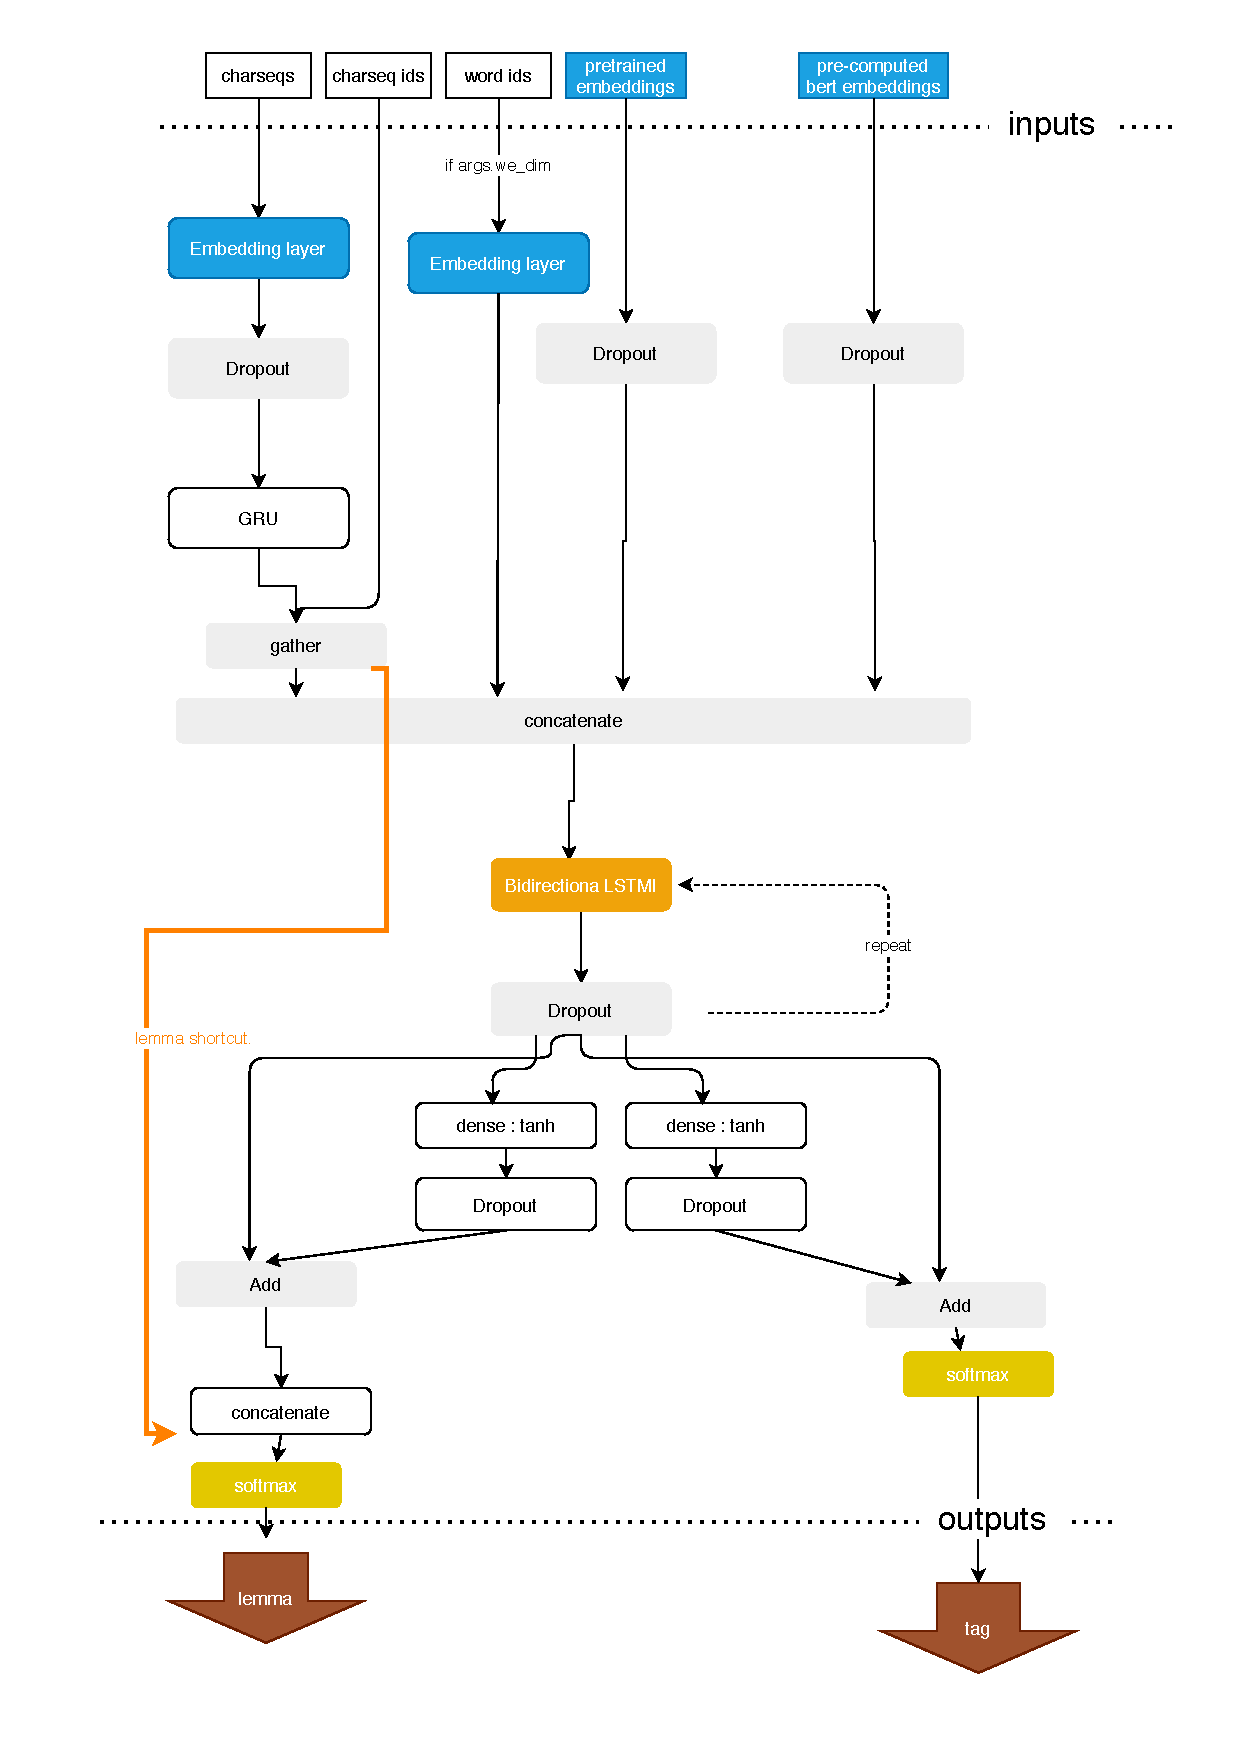
\includegraphics[width=1\columnwidth]{../img/taggermodel.pdf}
\protect\caption{Tagging and lemmatization joint model architecture.}
\label{pic:lt_arch}
\end{figure}
%TODO kolik je tech lstm a tak,vsechny dimenze (do tabulky)

%For POS tagging, we applied a straightforward model in the lines of Ling et al. (2015) – first rep- resenting each word with its embedding, contextu- alizing them with bidirectional RNNs (Graves and Schmidhuber, 2005), and finally using a softmax classifier to predict the tags. z UDpipe2

The model for lemmatization and tagging is build upon a model (and a code) for previous work on Czech NLP processing with contextual embedding \citep{Straka2019}. 
Data preprocessing is taken over from the paper as well as the structure of the lemmatizer and the tagger network, which is extended by BERT-like models, hoping for improvements. %TODO k tomu nemam citaci
Previous work showed that training tagging and lemmatization together in one network can be mutually advantageous, so both of these analyses are an output of one network, and are trained jointly. Detailed visualisation of network architecture can be found in figure \ref{pic:lt_arch}. \par The architecture of the network can be divided into three parts -- inputs, optional \acrshort{rnn}s, classification head:
\paragraph{Inputs}
An input set of the network consists of five different input types -- characters (charseqs), words (charseq ids), correct responses (word ids), pretrained embeddings, and possibly precomputed BERT embeddings (depending on the experiment type). Two other types of embeddings are created before the further processing of inputs by \acrshort{rnn} cells: character-level embeddings and another word embeddings that are, in contrast to BERT and pretrained embeddings, also trained during the training process.

\paragraph{RNN cells}
Character-level embeddings are further processed via 1 layer of \acrfull{gru} and all inputs (or their embeddings) are processed by recurrent part of network (specifically by three layers of \acrfull{lstm} cells).

\paragraph{Classification head(s)}
After the processing by recurrent neural networks, network employs two separate classification heads, one for tagging and another for lemmatization. Both heads use dense layer with tanh activation function to allow task-specific non-linear transformation as used in \citep{Straka2018} and a softmax function for obtaining the probability distribution over target classes. Lemmatization, however, presents another change -- addition of character level data without RNN processing, that are used together with the rest of the values as an input into the softmax following \citep{Straka2018}, as it leads to better performance of lemmatization in the case of shared network between both tasks.

%TODO kondraytuk bere predikci k prvnímu subwordu, jak to delam ja? 


\paragraph{Morphological Dictionary} All classification can be done with or without use of a morphological dictionary MorfFlex \citep{11234/1-1834}, that can provide possible pairs \textit{tag-lemma}. If used, the generated tag and lemma is a pair with maximal likelihood, but chosen just from the dictionary. This leads to more consistent results. 

%TODO maximal probability



%TODO nekde mam taky dropouts! zminit
\subsubsection{Experiments}
This part uses all main \textbf{experiment types} as decribed in \ref{sec:expe}: \textit{base, ls, embed, fine, simple}, and \textit{full}. Three \textbf{BERT-like models} are used for experiment setup:
\begin{itemize}
\item multilingual BERT (mBERT) \citep{Devlin2019}, 
\item XLM-RoBERTa \citep{Conneau2019}, 
\item RobeCzech \citep{Straka2021}.
\end{itemize}
XLM-RoBERTa and mBERT are trained on 100/104 different languages including Czech. RobeCzech is a recently published version of RoBERTa, trained only on Czech data. XLM-RobERTa is used only for embedding and one version of fine-tuning, and this model was omitted in other experiements because of weak results and high computational complexity. There exists another monolingual Czech model, Czert \citep{Sido2021}, which uses the original BERT architecture and was outperformed by RobeCzech \citep{Straka2021}. \par
A selection of layers is made in both ways -- last four layers (\textit{four)} and learning of weighted sum of all layers (\textit{att}). The layer attention is made only for the fine-tuning setup, and as the weighted sum does not show a significant benefit, mean of the last four layer is the only method used for other experiments.
 \par Learning rate is used as usual for each type of task and three different learning rate schedules were applied in each combination of hyperparameters: cosine decay \textit{(cos)}, inverted square root decay \textit{(isrd)} and a one epoch warm-up followed by a constant learning rate \textit{(warmup)} inspired by \citep{Kondratyuk2019} and \citep{Ruder2018}. For \textit{embed} experiments, \textit{warmup} is replaced by  a simple division of training into two parts with different learning rates. 
 
 \begin{table}[!h]
 \centering
\begin{tabular}{|l||l|}
\hline
hyperparametr   & \multicolumn{1}{l|}{value} \\ \hline \hline
beta\_2          & 0.99                       \\ \hline
optimizer       & Adam                       \\ \hline
cle\_dim         & 256                        \\ \hline
dropout         & 0.5                        \\ \hline
label smoothing & 0.3                        \\ \hline
rnn\_cell        & LSTM                       \\ \hline
rnn\_cell\_dim    & 512                        \\ \hline
rnn\_layers      & 3                          \\ \hline
we\_dim          & 512                        \\ \hline
word\_dropout    & 0.2                        \\ \hline
batch size & 64 \\ \hline
\end{tabular}
\caption[Hyperparameters of tagging and lemmatization common to all experiments]{Hyperparameters of tagging and lemmatization common to all experiments (if they make sense in the context of experiments).}
\label{tab:hyp_all}
\end{table}
Batches have size 64, given by the compromise between the pursuit of relatively big batch size and computational resources. Summary of hyperparameters, which do not differ across experiments is presented in table \ref{tab:hyp_all}. Other hyperparameters for each experiment are in table \ref{att:1}.
\par 
Reimplementation of \citep{Straka2019a} without any BERT-like model incorporation serves as a baseline.

\subsection{Results and Discussion}
Best presented model (experiment no. 18) achieved the same or better results than the current \acrlong{sota} tagging and lemmatization results (table \ref{tab:all_prew}). Complete results are in table \ref{tab:all_res_tl}. Experiment \textit{tl\_18} is the version with fine-tuning, Czech monolingual model, RobeCzech, and without layer attention, although the difference from comparable experiment with layer attention is insignificant and can be just accidental. The dominance of the Czech model was expected and additional expert knowledge contained in the complicated architecture was also assumed to be better. Experiments also showed that fine-tuning approach achieves better results than full training from the beginning. This may be due to the choice of hyperparameters, especially the learning rate, but the standard ones were selected, implying that at best, it is more difficult to find the right parameters for\textit{full} and \textit{simple} variants. Although \textit{simple} experiments presents standard approach of using pretrained BERT models, they turned out being less successful even than \textit{embed} experiments, that are faster to train and less memory intensive. 

\begin{table}[!h]
\centering
  \resizebox{\columnwidth}{!}{\begin{tabular}{|l||ccc||ccc|}
  \hline
\multirow{2}{*}{Experiment} & \multicolumn{3}{c||}{Without Dictionary}  &
      \multicolumn{3}{c|}{With Dictionary} \\ 
    & Tags & Lemmas & Both & Tags & Lemmas & Both \\ \hline \hline
    \textit{\citep{Straka2019}} & \textit{97.94} & \textit{98.75} & \textit{97.31} & \textit{98.05} & \textit{98.98} & \textit{97.65 }\\ \hline
   \textit{ StrakaC} & \textit{97.67} & \textit{98.63} & \textit{97.02} & \textit{97.91 }& \textit{98.94} & \textit{97.51} \\ \hline
     \textit{RobeCzech} & \textit{98.43} & \textit{98.79}  & \textit{97.83}  & \textit{98.50} & \textit{\textbf{99.00}}  & \textit{98.11} \\ \hline \hline
      baseline & 97.04  & 98.56  & 96.41 &  97.31   & 98.83  & 96.90 \\ \hline 
    emb(12) & 98.38  &98.79  & 97.80 & 98.48  & 98.99 & 98.10 \\ \hline
    best(18) & \textbf{98.50}  & \textbf{98.80} &\textbf{ 97.90}  & \textbf{98.57}  & \textbf{99.00}  & \textbf{98.19}  \\ \hline  
  \end{tabular}}
  \caption[Comparison of our best results and previous work]{
  \textit{Straka2019C} is a comparable solution  (BERT embeddings only) from \citep{Straka2019} to \textit{emb}, which was transformed into Tensorflow 2 in this work as a \textit{baseline}. \textit{Emb} is a solution with static BERT embeddings and \textit{best(18) is the best resulting model in this thesis (experiment id = 18). }}
\label{tab:all_prew} 
\end{table}


%TODO vsechny Figure a table se stejnym pismenem

\begin{table}[!h]
\resizebox{\columnwidth}{!}{
\begin{tabular}{|l|l|l|l|l|l||llllll|}
\hline
\multicolumn{2}{|c|}{\multirow{2}{*}{Model}} &
  \multirow{2}{*}{EXPE} &
  \multirow{2}{*}{EP} &
  \multirow{2}{*}{LAYERS} &
  \multirow{2}{*}{LR} &
  \multicolumn{2}{c}{Lemmas} &
  \multicolumn{2}{c}{Tags} &
  \multicolumn{2}{c|}{Both} \\
\multicolumn{2}{|l|}{} &  &  &  &  & Raw & Dict & Raw & Dict & Raw & Dict  \\ \hline \hline
0  & NA                           & base                    & A	& NA               & simple & 98.58  & 98.81   & 97.05   & 97.31    & 96.43     & 96.9       \\ \hline
1  & NA                           & ls                      & B	& NA               & simple & 98.55  & 98.81   & 97.12   & 97.34    & 96.51     & 96.94      \\ \hline
2  & \multirow{3}{*}{mBERT}       & \multirow{9}{*}{embed}  & B	& four             & simple & 98.69  & 98.93   & 97.83   & 97.98    & 97.17     & 97.58      \\ \cline{1-1} \cline{4-12}
3  &                              &                         & C	& four                     & cos    & 98.74  & 98.95   & 97.91   & 98.04    & 97.28     & 97.63      \\ \cline{1-1} \cline{4-12}
4  &                              &                         & C	& four                     & isrd   & 98.73  & 98.94   & 97.89   & 98.02    & 97.28     & 97.61      \\ \cline{1-2} \cline{4-12}
5  & \multirow{3}{*}{xlm-Roberta} &                         & B	& four             & simple & 98.57  & 98.8    & 97.33   & 97.54    & 96.68     & 97.12      \\ \cline{1-1} \cline{4-12}
6  &                              &                         & C	& four                     & cos    & 98.6   & 98.83   & 97.45   & 97.62    & 96.81     & 97.21      \\ \cline{1-1} \cline{4-12}
7  &                              &                         & C	& four                     & isrd   & 98.59  & 98.83   & 97.44   & 97.61    & 96.81     & 97.2       \\ \cline{1-2} \cline{4-12}
8  & \multirow{3}{*}{RoBECzech}   &                         & B	& four             & simple & 98.77  & 98.97   & 98.38   & 98.48    & 97.78     & 98.08      \\ \cline{1-1} \cline{4-12}
9  &                              &                         & C	& four                     & cos    & 98.79  & 98.99   & 98.38   & 98.48    & 97.80      & 98.10      \\ \cline{1-1} \cline{4-12}
10 &                              &                         & C	& four                     & isrd   & 98.78  & 98.98   & 98.4    & 98.48    & 97.8      & 98.09      \\ \hline
11 & \multirow{3}{*}{mBERT} & \multirow{9}{*}{fine}         & D	& four     & simple & 98.69 & 98.93 & 97.84 & 97.99 & 97.21 & 97.59 \\ \cline{1-1} \cline{4-12}
12 &                              &                         & E	& four             & cos    & 98.72  & 98.95   & 97.97   & 98.08    & 97.33     & 97.68      \\ \cline{1-1} \cline{4-12}
13 &                              &                         & E	& four             & isrd   & 98.68  & 98.9    & 97.72   & 97.86    & 97.09     & 97.46      \\ \cline{1-2} \cline{4-12}
14 & \multirow{3}{*}{xlm-Roberta} &                         & D	& four     & simple & 98.62  & 98.84   & 97.72   & 97.9     & 97.07     & 97.48      \\ \cline{1-1} \cline{4-12}
15 &                              &                         & E	& four             & cos    & 98.67  & 98.9    & 97.95   & 98.09    & 97.32     & 97.69      \\ \cline{1-1} \cline{4-12}
16 &                              &                         & E	& four             & isrd   & 98.63  & 98.85   & 97.66   & 97.83    & 97.03     & 97.41      \\ \cline{1-2} \cline{4-12}
17 & \multirow{3}{*}{RoBECzech}   &                         & D	& four     & simple & 98.78  & 98.98   & 98.46   & 98.55    & 97.86     & 98.16      \\ \cline{1-1} \cline{4-12}
18 &                              &                         & E	& four             & cos    & \textbf{98.80}   & \textbf{99.00 }     & \textbf{98.50}    & \textbf{98.57}    & \textbf{97.90 }     & \textbf{98.19 }     \\ \cline{1-1} \cline{4-12}
19 &                              &                         & E	& four             & isrd   & 98.76  & 98.95   & 98.33   & 98.41    & 97.72     & 98.02      \\ \cline{1-2} \cline{4-12} \hline
20 & \multirow{3}{*}{mBERT}  &  \multirow{9}{*}{fine att}   & D	& att                       & simple & 98.67  & 98.91   & 97.76   & 97.92    & 97.13     & 97.52      \\ \cline{1-1} \cline{4-12}
21 &                              &                         & E	& att              & cos    & 98.72  & 98.95   & 97.98   & 98.1     & 97.34     & 97.69      \\ \cline{1-1} \cline{4-12}
22 &                              &                         & E	& att              & isrd   & 98.67  & 98.91   & 97.69   & 97.85    & 97.05     & 97.45      \\ \cline{1-2} \cline{4-12}
23 & \multirow{3}{*}{xlm-Roberta} &                         & D	& att      & simple & 98.6   & 98.81   & 97.62   & 97.77    & 96.96     & 97.35      \\ \cline{1-1} \cline{4-12}
24 &                              &                         & E	& att              & cos    & 98.67  & 98.89   & 97.91   & 98.06    & 97.29     & 97.66      \\ \cline{1-1} \cline{4-12}
25 &                              &                         & E	& att              & isrd   & 98.65  & 98.86   & 97.65   & 97.81    & 97.03     & 97.41      \\ \cline{1-2} \cline{4-12}
26 & \multirow{3}{*}{RoBECzech}   &                         & D	& att      & simple & 98.77  & 98.97   & 98.38   & 98.47    & 97.79     & 98.08      \\ \cline{1-1} \cline{4-12}
27 &                              &                         & E	& att              & cos    & \textbf{98.8}   & 98.99   & 98.47   & 98.54    & 97.88     & 98.16      \\ \cline{1-1} \cline{4-12}
28 &                              &                         & E	& att              & isrd   & 98.77  & 98.96   & 98.33   & 98.41    & 97.72     & 98.01      \\ \hline
29 & \multirow{3}{*}{mBERT}       & \multirow{9}{*}{simple} & F	& four                     & warmup & 98.17  &         & 97.32   &          & 96.46     &            \\ \cline{1-1} \cline{4-12}
30 &                              &                         & G	& four                     & cos    & 98.15  &         & 97.39   &          & 96.47     &            \\ \cline{1-1} \cline{4-12}
31 &                              &                         & G	& four                     & isrd   & 98.13  &         & 97.12   &          & 96.29     &            \\ \cline{1-2} \cline{4-12}
35 & \multirow{3}{*}{RoBECzech}   &                         & F	& four                     & warmup & 98.49  &         & 98.28   &          & 97.41     &            \\ \cline{1-1} \cline{4-12}
36 &                              &                         & G	& four                     & cos    & 98.46  &         & 98.30   &          & 97.39     &            \\ \cline{1-1} \cline{4-12}
37 &                              &                         & G	& four                     & isrd   & 98.59  &         & 98.27   &          & 97.53     &            \\ \hline
38 & \multirow{3}{*}{mBERT}       & \multirow{9}{*}{full}   & F	& four                     & warmup & 98.16  & 98.86   & 97.35   & 97.79    & 96.46     & 97.34      \\ \cline{1-1} \cline{4-12}
39 &                              &                         & G	& four                     & cos    & 98.04  & 98.85   & 97.36   & 97.81    & 96.3      & 97.34      \\ \cline{1-1} \cline{4-12}
40 &                              &                         & G	& four                     & isrd   & 98.22  & 98.86   & 97.34   & 97.73    & 96.46     & 97.29      \\ \cline{1-2} \cline{4-12}
44 & \multirow{3}{*}{RoBECzech}   &                         & G	& four                     & warmup & 98.49  & 98.95   & 98.21   & 98.34    & 97.38     & 97.93      \\ \cline{1-1} \cline{4-12}
45 &                              &                         & G	& four                     & cos    & 98.25  & 98.95   & 98.17   & 98.33    & 97.08     & 97.89      \\ \cline{1-1} \cline{4-12}
46 &                              &                         & G	& four                     & isrd   & 98.55  & 98.99   & 98.19   & 98.35    & 97.39     & 97.95      \\ \hline

\end{tabular}
}
\caption[Complete results for tagging and lemmatization]{This table presents complete results for tagging and lemmatizationt tasks. Column EP presents number of epochs and corresponding learning rates are explained in Attachement \protect\ref{att:1} }
\label{tab:all_res_tl}
\end{table}

\subsubsection{Error Analysis}
%TODO sjednotit názvy modelů
This section offers a little exploration of differences in error across models. This comparison includes three models: 
\begin{itemize}
\item tl\_18 -- the best model in tagging and lemmatization,
\item tl\_3 -- the best model with mBERT,
\item tl\_1 -- the baseline model with label smoothing.
\end{itemize} 

\paragraph{best vs. baseline}
The best model (tl\_18) improves prediction in $3,247$ tags and is worse in 421 tag predictions. More than 80\% of newly correctly predicted tags are composed by three parts of speech: NN (noun), AA (adjective), and RR (preposition). Table \ref{att:tags1} presents improved tags with a frequency at least 10. The most frequent tag ( \texttt{NNIS1-----A----}) presents proper names of places (e.g. Jersey, Tenesee), but we can see that other frequent tags are nominatives and accusatives of masculinum, singular,  inainamate (cs: \textit{rod mužský neživotný}) or femininum, plural. These two cases have the same form for mentioned categories, so they are indistinguishable without context, and that is where BERT showed to be very useful. The same situation is with adjectives, again mostly nominative or accusative of the same form, for example words \textit{další} (following) or \textit{stínový} (shadowy). The third category are prepositions that can be connected with both accusative and dative as \textit{na} (on), or \textit{o} (about).

%TODO kolik lemmata

\paragraph{mBERT vs. RobeCzech}
Best mBERT is better in 468 tags and worse in $1,703$ tags than the best model. The most frequent tags improved by \textit{tl\_18} are similar to previous comparison. Nominative and accusative are again the most common cases improved, but the differences between these two models are not so significant. This results in verbs appearing higher in the table of most frequent tags, although the absolute value of better predictions on verbs is similar to previous comparison. In both situations, improved verbs predictions relate mostly to verbs with the same form in singular and plural of the third-person, e.g. \textit{vyváží} (exports) or \textit{stojí} (stands). The complete table of the most frequent tags is available in table \ref{att:tags2}.
%TODO kolik lemmata
%TODO je v necem mBERT lepsi?

\newpage
\section{Sentiment Analysis}
\label{chap:sent}
As stated in \citep{Veselovska}: "Sentiment analysis, also known as opinion mining, is an automatic detection of a positive or negative polarity, or neutrality of ... a text sequence", which is exactly as the sentiment analysis is understood in this work, although there are some other definitions consisting of e.g. opinion extraction, irony or stance \citep{Montoyo2012}. Another tasks related to sentiment analysis is a subjectivity analysis (whether the presented opinion is objective or highly subjective), which is also not included in this work, mainly because the lack of labelled data for Czech. It is possible to analyze individual expressions, sentences or whole documents \citep{Veselovska} and this work focuses on the document level classification.
\subsection{Task definition}
\paragraph{Sentiment analysis} \mbox{}\\
\textit{input:} sequence of sentences (a whole post or comment, depending on the source) \\
\textit{output:} prevailing sentiment of the input from categories: neutral, positive, negative.
\par

\paragraph{Metric} For evaluating performance, two metrics are used: macro-averaged F1 score and accuracy. Both metrics are chosen for better comparability with previous work.

\subsection{Related Work}
citace:
\citep{Cano2019}
\citep{Kittask2020} .. estonian
\citep{Lenc2016} sentiment in czech
\citep{Hercig2018}
\citep{Li}
\citep{Libovicky} presents state-of-the art results in three czech NLP tasks including sentiment analysis. They use only CSFD dataset with resulting accuracy 80.8 .1 which is still not so good as Brychcín (81.5.3). The second mentioned paper, however, uses quite complicated method for classification incorporating the fact of which movie is reviewed. 

Bachelor thesis which aplies bert on sentiment analysis in czech:
%https://dspace.cvut.cz/bitstream/handle/10467/83127/F8-BP-2019-Langr-Lukas-thesis.pdf?sequence=-1&isAllowed=y
results are accuracy 84 with tfidf and about 81 with bert and they used mall dataset.

\subsection{Dataset and Preprocessing}
%TODO zjistit jaka jsou na to porovnavaci data This work primary tries to improve existing tasks and show the ability of contextualized embeddings to improve results, so tasks with existing data and results were selected.  %TODO why?
Four main Czech datasets with sentiment annotation are available: user reviews from MALL.cz (mall), film reviews from csfd.cz (csfd), news from Aktualne.cz (aktualne) and posts from czech branch pages on facebook.cz (facebook). As \textit{aktualne} dataset turned out to be problematical because the text were ambiguous even for annotators, and its authors later used other mentioned datasets \citep{Veselovska}, this work also focuses only on the three other data sources -- \textit{mall}, \textit{csfd} and \textit{facebook} \footnote{All three datasets are all available here: http://liks.fav.zcu.cz/sentiment/}. Some experiment are also performed with in-domain training on Eglish data. For this purpose is used \textit{imdb} dataset \footnote{https://www.tensorflow.org/datasets/catalog/imdb\_reviews}, which contains movie review from the biggest movie rating website imdb.com. This leads to some problems described later in this section, because English dataset contains only binary classification (positive/negative). Table \ref{tab:datasets} summarize each dataset.
%TODO popis tabulky
\begin{center}
\begin{table}[]
\begin{tabular}{|l||lll|}
\hline
     & length & labels                                                                & domain        \\ \hline \hline
\textbf{mall}     & 145306 & \begin{tabular}[c]{@{}l@{}}positive\\ neutral\\ negative\end{tabular} & domestic appliance reviews                             \\ \hline
\textbf{csfd} & 91304  & \begin{tabular}[c]{@{}l@{}}positive\\ neutral\\ negative\end{tabular} & movie reviews \\ \hline
\textbf{facebook} & 9752   & \begin{tabular}[c]{@{}l@{}}positive\\ neutral\\ negative\end{tabular} & \begin{tabular}[c]{@{}l@{}}brand pages of e.g. shops or mobile networks \\ providers\end{tabular} \\ \hline
\textbf{imdb} & 25000  & \begin{tabular}[c]{@{}l@{}}positive\\ negative\end{tabular}           & movie reviews \\ \hline
\end{tabular}
\label{tab:datasets}
\caption{Three Czech datasets (mall, facebook, csfd) and one English (imdb) are used for training in this work.}
\end{table}
\end{center}


%TODO je to rozdleeno se stratifikací?
%TODO popis obrazku
\begin{figure}[!ht]
\centering
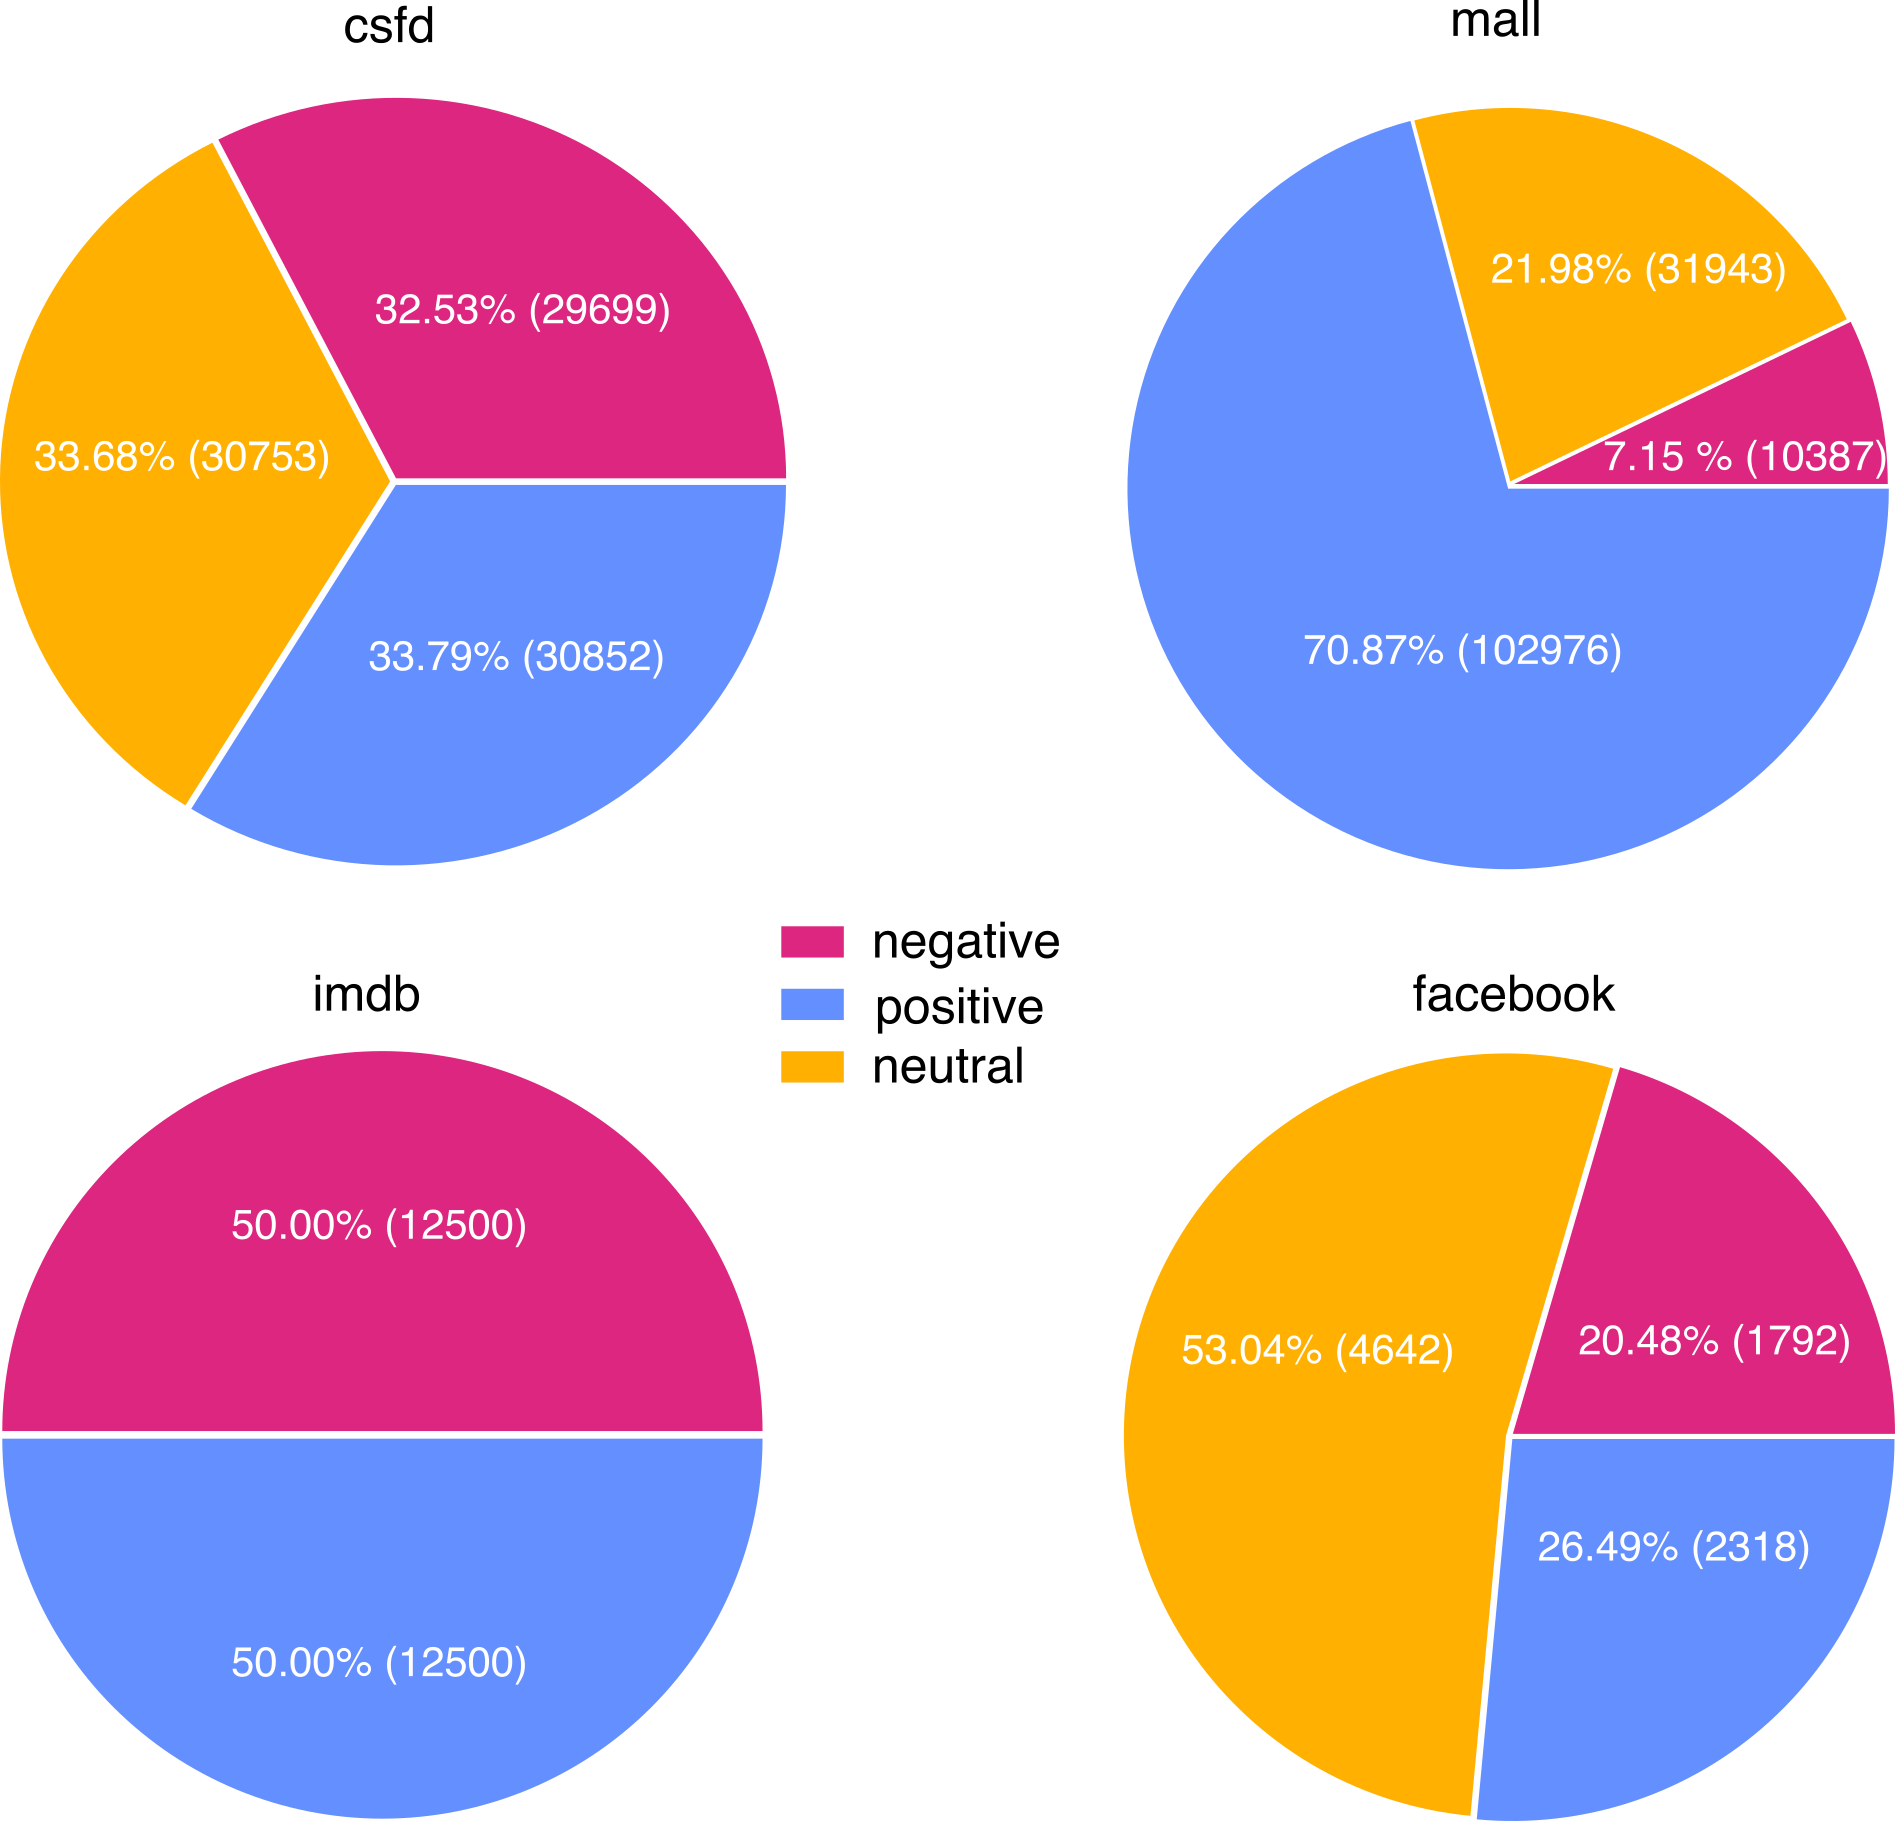
\includegraphics[width=1\columnwidth]{../img/dist_all.png}
\protect\caption{Distribution of positive/neutral/negative labels in each dataset.}
\label{pic:dist}
\end{figure}

As can be seen in figure \ref{pic:dist}
distribution of labels differs among datasets. Moreover, Figure \ref{pic:dist_all}
\begin{figure}[!ht]
\centering
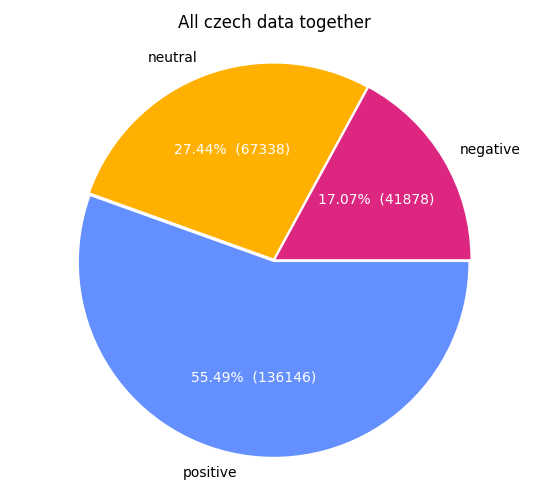
\includegraphics[width=0.7\columnwidth]{../img/all.png}
\protect\caption{Percentage and absolute values of labels in all three Czech datasets together.}
\label{pic:dist_all}
\end{figure}
%TODO all má blbý nadpis
shows, that the resulting dataset is highly unbalanced, which causes divergence and stuck in training. Due to the big part of labels being positive, many learning strategies just ended with predicting only \textit{positive} class, i.e. 55\% accuracy, so unfortunately learned nothing. 

%This was the the case for following experiments settings:
%learning rate of $2e-3$ for 10 epochs. This ended with predicting only one class (positive). Some progress showed the followign approach:"2:5e-5,1:2e-5, unfreezed" for facebook data only (which are balanced). This results are above 71 for accuracy (Test accuracy: 0.726
%F1 metrics: 0.7077061630227595 weighted).


\subsection{Experiments and Architecture}
The main division of experiments is by the input dataset -- each of Czech models separately and one joint dataset consisting of all Czech datasets, i.e. four different datasets. All variants performed both layers attention and an average of last four layers. As for the learning rate, all experiments were made with learning rate $3 \times 10^{-5}$ and there were always two types of learning rate decay -- cosine and inverse square root decay. 
\par
Network architecture is much simpler than in tagging and lemmatization task and corresponds to \textit{simple} setting of these tasks -- only BERT-like model and classification head consisting of layer with softmax activation function. %TODO a neni tam nahodou jeste neco?

\begin{figure}[h]
\centering
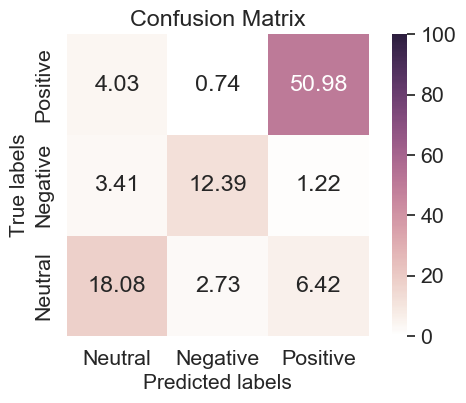
\includegraphics[width=1\columnwidth]{../img/confusion_matrix}
\protect\caption{Normalized confusion matrix}
\label{pic:conf1}
\end{figure}

\subsection{Results and Discussion}
%I tried another approach:
%Because the facebook dataset is balanced, I pretrained the model first on facebook and after reaching a decent accuracy, i further trained the model on the join data:
%for ten epochs with learning rate 5e-5 and an effecctive batch size 48.
%[[ 6240 914 2783]
%[ 1236 4447 529]
%[ 1050 273 19020]]
%Test accuracy: 0.814068837005371
%F1 metrics: 0.8087903170140932

%The pretraining model was obtained as:
%without freezing, batch size 48, 2:5e-5,4:2e-5



%Than I trained for 3 more epochs:
%[[ 6599 995 2343]
%[ 1246 4520 446]
%[ 1470 269 18604]]
%Test accuracy: 0.8145072892688808
%F1 metrics: 0.8119431050948791
%TODO  \ref{pic:conf1}

Baseline for this task is tf-idf method %TODO nekde je popsana v prni kapitole
, which resulted in 
[[ 4310   102  3015]
 [  685  1016   779]
 [  842    48 20227]]
              precision    recall  f1-score   support

           0       0.74      0.58      0.65      7427
           1       0.87      0.41      0.56      2480
           2       0.84      0.96      0.90     21117

    accuracy                           0.82     31024
   macro avg       0.82      0.65      0.70     31024
weighted avg       0.82      0.82      0.81     31024


% Please add the following required packages to your document preamble:
% \usepackage{multirow}
\begin{table}[]
\resizebox*{!}{\textheight}{\begin{tabular}{|l|l|l|l||ll|}
\hline
\multicolumn{2}{|l|}{MODEL}       & EXPE                      & LRTYPE                & Acc    & F1   \\ \hline  \hline
1  & \multirow{6}{*}{mBERT}     & czech                     & \multirow{3}{*}{Isrd} & 0,81   & 0,81 \\ \cline{1-1} \cline{3-3} \cline{5-6} 
2  &                            & zero                      &                       & 0,50   & 0,45 \\ \cline{1-1} \cline{3-3} \cline{5-6} 
3  &                            & eng                       &                       & 0,81   & 0,81 \\ \cline{1-1} \cline{3-6} 
4  &                            & czech                     & \multirow{3}{*}{cos}  & 0,83   & 0,82 \\ \cline{1-1} \cline{3-3} \cline{5-6} 
5  &                            & zero                      &                       & 0,53   & 0,48 \\ \cline{1-1} \cline{3-3} \cline{5-6} 
6  &                            & eng                       &                       & 0,83   & 0,82 \\ \hline
13 & \multirow{4}{*}{RoBECzech} & czech                     & \multirow{2}{*}{isrd} & 0,81   & 0,81 \\ \cline{1-1} \cline{3-3} \cline{5-6} 
14 &                            & zero                      &                       & 0,55   & 0,48 \\ \cline{1-1} \cline{3-6} 
16 &                            & czech                     & \multirow{2}{*}{cos}  & 0,84   & 0,84 \\ \cline{1-1} \cline{3-3} \cline{5-6} 
17 &                            & zero                      &                       & 0,58   & 0,49 \\ \hline
19 & \multirow{6}{*}{mBERT}     & czech                     & \multirow{3}{*}{Isrd} & 0,82   & 0,81 \\ \cline{1-1} \cline{3-3} \cline{5-6} 
20 &                            & zero                      &                       & 0,54   & 0,48 \\ \cline{1-1} \cline{3-3} \cline{5-6} 
21 &                            & eng                       &                       & 0,82   & 0,81 \\ \cline{1-1} \cline{3-6} 
22 &                            & czech                     & \multirow{3}{*}{cos}  & 0,83   & 0,82 \\ \cline{1-1} \cline{3-3} \cline{5-6} 
23 &                            & zero                      &                       & 0,52   & 0,47 \\ \cline{1-1} \cline{3-3} \cline{5-6} 
24 &                            & eng                       &                       & 0,83   & 0,82 \\ \hline
31 & \multirow{4}{*}{RoBECzech} & czech                     & \multirow{2}{*}{isrd} & 0,83   & 0,83 \\ \cline{1-1} \cline{3-3} \cline{5-6} 
32 &                            & zero                      &                       & 0,58   & 0,50 \\ \cline{1-1} \cline{3-6} 
34 &                            & czech                     & \multirow{2}{*}{cos}  & 0,84   & 0,84 \\ \cline{1-1} \cline{3-3} \cline{5-6} 
35 &                            & zero                      &                       & 0,58   & 0,51 \\ \hline
37 & \multirow{2}{*}{mBERT}     & \multirow{7}{*}{facebook} & Isrd                  & 0,75   & 0,75 \\ \cline{1-1} \cline{4-6} 
38 &                            &                           & cos                   & 0,76   & 0,76 \\ \cline{1-2} \cline{4-6} 
41 & \multirow{5}{*}{RoBECzech} &                           & isrd                  & 0,80   & 0,80 \\ \cline{1-1} \cline{4-6} 
42 &                            &                           & simple                & 0,79   & 0,79 \\ \cline{1-1} \cline{4-6} 
43 &                            &                           & \multirow{3}{*}{cos}  & 0,82   & 0,81 \\ \cline{1-1} \cline{5-6} 
44 &                            &                           &                       & 0,81   & 0,81 \\ \cline{1-1} \cline{5-6} 
45 &                            &                           &                       & 0,82 & 0,82 \\ \hline
46 & \multirow{2}{*}{mBERT}     & \multirow{4}{*}{facebook} & Isrd                  & 0,76   & 0,76 \\ \cline{1-1} \cline{4-6} 
47 &                            &                           & cos                   & 0,77   & 0,77 \\ \cline{1-2} \cline{4-6} 
50 & \multirow{2}{*}{RoBECzech} &                           & isrd                  & 0,80   & 0,79 \\ \cline{1-1} \cline{4-6} 
51 &                            &                           & cos                   & 0,806  & 0,80 \\ \hline
52 & \multirow{2}{*}{mBERT}     & \multirow{8}{*}{mall}     & Isrd                  & 0,83   & 0,83 \\ \cline{1-1} \cline{4-6} 
53 &                            &                           & cos                   & 0,84   & 0,84 \\ \cline{1-2} \cline{4-6} 
56 & \multirow{2}{*}{RoBECzech} &                           & isrd                  & 0,83   & 0,83 \\ \cline{1-1} \cline{4-6} 
57 &                            &                           & cos                   & 0,85   & 0,84 \\ \cline{1-2} \cline{4-6} 
58 & \multirow{2}{*}{mBERT}     &                           & Isrd                  & 0,83   & 0,83 \\ \cline{1-1} \cline{4-6} 
59 &                            &                           & cos                   & 0,84   & 0,84 \\ \cline{1-2} \cline{4-6} 
62 & \multirow{2}{*}{RoBECzech} &                           & isrd                  & 0,84   & 0,84 \\ \cline{1-1} \cline{4-6} 
63 &                            &                           & cos                   & 0,85   & 0,84 \\ \hline
64 & \multirow{2}{*}{mBERT}     & \multirow{8}{*}{csfd}     & Isrd                  & 0,81   & 0,81 \\ \cline{1-1} \cline{4-6} 
65 &                            &                           & cos                   & 0,82   & 0,82 \\ \cline{1-2} \cline{4-6} 
68 & \multirow{2}{*}{RoBECzech} &                           & isrd                  & 0,83   & 0,83 \\ \cline{1-1} \cline{4-6} 
69 &                            &                           & cos                   & 0,85   & 0,85 \\ \cline{1-2} \cline{4-6} 
70 & \multirow{2}{*}{mBERT}     &                           & Isrd                  & 0,82   & 0,82 \\ \cline{1-1} \cline{4-6} 
71 &                            &                           & cos                   & 0,82   & 0,82 \\ \cline{1-2} \cline{4-6} 
74 & \multirow{2}{*}{RoBECzech} &                           & isrd                  & 0,83   & 0,83 \\ \cline{1-1} \cline{4-6} 
75 &                            &                           & cos                   & 0,84   & 0,84 \\ \hline
\end{tabular}}
\end{table}



%Because BERT model was trained on multilingual data, it is naturally not so good in language minoritly presented in the Bert's training data. When transfering the learned knowledge to czech sentiment task, we actually want to improve model in two ways: teach it something more specific about given task, i.e., sentiment, and improve its knowledge about selected language (czech in this case). By using czech sentiment dataset, both thing are incorporated into training. To obtained better results and following the \citep{Putra}, I also selected english sentiment dataset. The idea behind is that BERT is quite good in english and maybe can learn faster useful knowledge about the given task from data in more familiar language.















%\section{Lemmatization and part-of-speech tagging}
\label{chap:tag}
Lemmatization and \acrshort{pos} tagging tasks are categorized as morphological analysis, share the same architecture and trained network and they will be described together in this section.
\subsection{Task Definition}

\paragraph{\textbf{POS tagging}} \mbox{}\\
\textit{input}: a sequence of  words \\
\textit{output}: tag (for each word), which contains not only part-of-speech (e.g. noun, pronoun, punctuation mark) but also other morphological analysis (case, tense, etc) corresponding to 15-places morphological tagging system by \cite{Hajic2004}. Description of each position can be found in table \ref{Tab:tagset}.

\paragraph{\textbf{Lemmatization}} \mbox{}\\
\textit{input:} a sequence of words \\
\textit{output:} lemma (for each word) -- a base form of a given words, for example nominative of singular for nouns or infinitive for verbs. In this work, lemmatization is treated as a classification problem with classes coresponding to generating rules which transform an input word into target lemma. For example of such rules see figure \ref{fig:lemma_rules}. \\

\begin{table}[!ht]
\centering
\begin{tabular}{ |c|c|c| } 
 \hline
 Position & Name & Description \\ 
 \hline \hline
 1 & POS & Part of speech \\ \hline
 2 & SubPOS & Detailed part of speech \\ \hline
  3 & Gender & Gender \\ \hline
4 & Number & Number \\\hline
  5 & Case & Case \\ \hline
 6 & PossGender & Possessor's gender \\\hline
  7 & PossNumber & Possessor's number \\ \hline
8 & Person & Person \\\hline
  9 & Tense & Tense \\ \hline
 10 & Grade & Degree of comparison\\\hline
  11 & Negation & Negation \\ \hline
 12 & Voice & Voice \\\hline
 13 & Reserve1 & Reserve \\ \hline
14 & Reserve2 & Reserve \\\hline
  15 & Var & Variant, style \\ 
 \hline
\end{tabular}
\caption[Czech morphological tags]{Czech morphology developement is dated from 1989 \citep{Hajic2004} 
and in description of words uses 15-places morphological tags as described in this table taken from \url{https://ufal.mff.cuni.cz/pdt2.0/doc/manuals/en/m-layer/html/ch02s02s01.html}. For more detailed  description or for exploration of predictions given by this work is recommended to use website of Institute of Theoretical and Computational linguistics: \url{http://utkl.ff.cuni.cz/~skoumal/morfo/?pos=11\&val=1}, although they use slightly different set with additional 16 position. }
\label{Tab:tagset}
\end{table}

\paragraph{Metrics} Accuracy is used for the evaluation and is reported separately for several options -- only tags/lemmas, accuracy of joint classification of tags and lemmas, and  also all three variants with an usage of a morphological dictionary (this option is described in more detail in \ref{sub:dataset}).

\begin{figure}[!ht]
\centering
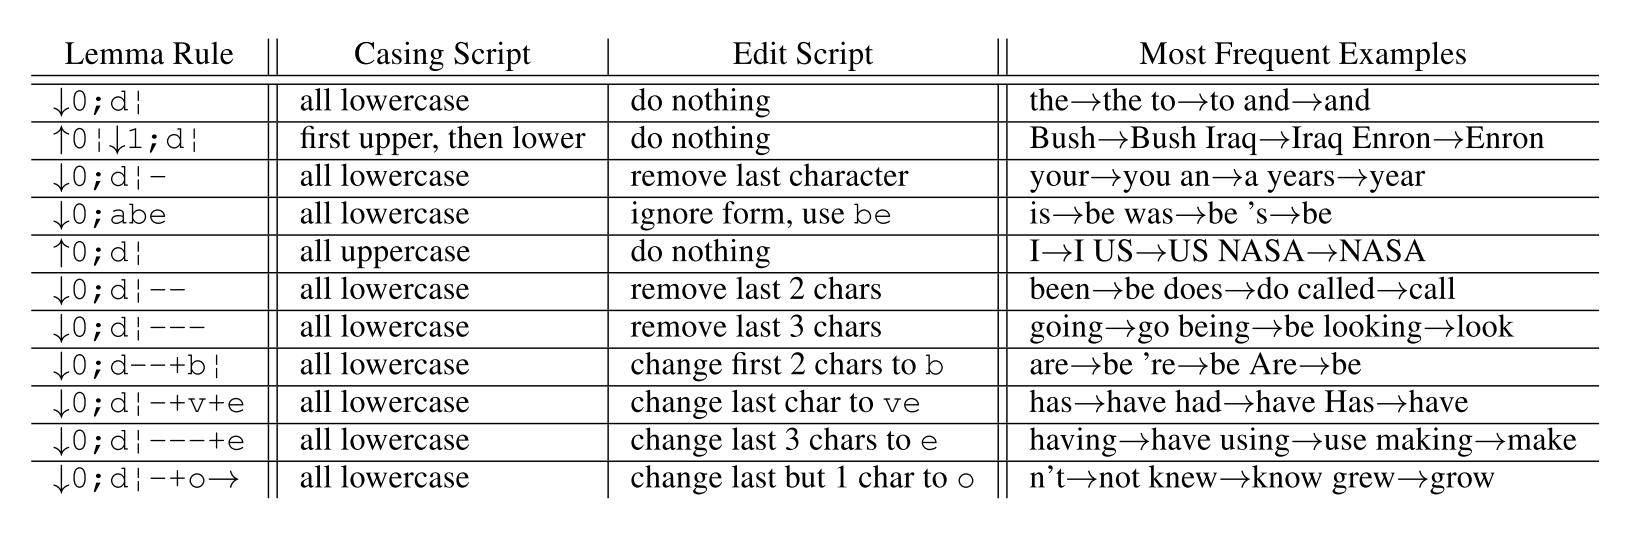
\includegraphics[width=1\textwidth]{../img/lemma_rules}
\protect\caption[The most common lemma generating rules in English EWT corpus]{
Table 1 from \citep{Straka2019b} presents 10 most common lemma generating rules in English EWT corpus. Each rule has two parts -- a casing script for transforming uppercase and lowercase letters, and an edit script. The edit script can transform prefix, suffix, or also a root of the word. It uses the Wagner–Fischer algorithm \citep{Wagner}, which finds the longest commont substring between the word and its lemma. Resulting rule is the shortest edit script converting the word into the lemma. More information can be found in \citep{Straka2019b}.
}
\label{fig:lemma_rules}
\end{figure}

\subsection{Related Work}
\subsubsection{Tagging}
This work aims to improve previously published SOTA results for contextualized embeddings in Czech lemmatization and tagging \citep{Straka2019} and \citep{Straka2021}. POS tagging (for English) is dated back to 1971 with first rule-based approach on Brown Corpus \citep{greene1971automatic}. Good results in POS tagging were achieved after year 2000 using both classical machine learning methods like Hidden Markov Models \citep{tnt} or Support Vector Machines \citep{svmtool}, and perceptrons/neural networks \citep{collins-2002-discriminative}. Actual English \acrshort{sota} known to me is presented in Flair model \citep{Akbik2018}.\footnote{More detailed overvirew of English tagging can be found here: https://aclweb.org/aclwiki/} It is necessary to note that early papers had \acrshort{pos} tagging defined differently than it is in this thesis. They focused only on selecting part of speech (noun, verb, etc...), meanwhile the later works (including this thesis) present complex morphological analysis.
\par
One of the first automatic tagging experiments in Czech is described in \citep{Hladka}, which also shows differences between languages with rich inflexion (as Czech,  but also Finnish or Turkish) and ones with simpler morphology (for example English or Spanish). Languages with complicated morphology have incomparably larger set of possible tags -- English has less then one hundred of possible tags, Czech has almost $4,000$ tags.  Current \acrshort{sota} results for tagging (and lemmatization) are presented in \citep{Straka2021}, which uses Czech version of RoBERTa model -- RobeCzech. This is the model also used for some experiments in this work and, as expected,  yields the best results. RobeCzech is based upon previous successful morphological analysis with contextual embeddings and BERT-like models \citep{Straka2019b}, \citep{Straka2019a}, \citep{Straka2019}, \citep{Straka2018} (all lastly mentioned models also achieved great results in lemmatization). \par
Although tagging is mostly considered to be a classification into predifined set of tags, the sets themselves can vary. Penn treebank uses a tagset of 54 different tags, which presents parts of speech and additional information like tense or number.\footnote{see: \url{https://www.sketchengine.eu/penn-treebank-tagset/}} There are some differences between this tagset and other English datasets or taggers (e.g., TreeTagger \citep{Schmid95improvementsin} or CLAWS tagset \citep{Chapelle1988TheCA}). All English tagsets are really small compared to languages like Czech or Turkish. As mentioned before, Czech uses 15-positioning tags, which is a natural solution for such type of languages. These positions can be predicted together or for each position separately. The first approach creates big tagset but guarantees consistency among positions (e.g. there will be no tense for a noun or a case for a verb). In the case of separate prediction, each position can be treated as a classification problem separately, which causes problems, because the individual parts of tag are not independent. Better approach is to use sequence-to-sequence modelling \citep{Sutskever2014}, which outputs the tag as a sequence of positions and takes into account previously generated position as in \citep{malaviya-etal-2019-simple}.

\subsubsection{Lemmatization}
Lemmatization (both Czech and English) has undergone a similar development as tagging, starting with rule-based approaches and statistical approaches \citep{Plisson}, continuing with neural networks and recently achieving good results with BERT-like models \citep{Kondratyuk2019}.  Lemmatization is typically performed as a sequence-to-sequence model, therefore it takes a word as a sequence of characters and produces a new sequence of characters, which is the lemma. This approach is teoretically better than classification into rules, because it is possible to generate every existing lemma. However, it can generate simply every possible character sequence, which may not be an existing word. Lemmatization as a classification task into edit scripts set firstly appeared in \citet{Chrupala} and was explored further by \citet{Straka2018}. 
Sequence-to-sequence model can be also used for production of edit rules (same rules as used in this work)\citep{chakrabarty2017context}, \citep{muller2015joint} and \citep{Yildiz2019}.

\subsection{Dataset and Preprocessing}
\label{sub:dataset}
Dataset for these tasks is taken from data of Prague Dependency Treebank (PDT) \citep{PDT35}, version 3.5 from year 2018. Data consists of sentences with lemmas and tags. For ambiguous words, data contain all possible analyses, which were generated using morphoDita \citep{Strakova} and morphological dictionary \citep{11234/1-1834} (described later).\footnote{genarator of analyses is available online: \url{https://lindat.mff.cuni.cz/services/morphodita/}.} For example, Czech word "psa" has one possible lemma ("pes") but two possible tags, because it could be one of two possible grammatical cases -- genitive or accusative. Input data for such word looks as follows: \\
\begin{center}
\texttt{psa pes NNMS2-----A---- NNMS4-----A----}.
\end{center}
Data contains about 1,600 unique tags and about 1,500 different lemma rules. The number of lemmas is significantly smaller than a number of unigue lemmas ($72,000$) \citep{Strakova} or tags, because words with similar morphological function have same way of creating lemma from the word, e.g. words \textit{malého} (=little, accusative,  sg, m.,) and \textit{červeného}  (=red, accusative,  sg, m.,) have the same lemma rule:
\begin{center}
\texttt{$\downarrow$ 0;d\textbrokenbar ---+ý+-+1}.
\end{center} 
\par
Dataset is originally divided into tree parts - train, development and test, which is also used in this work. Input sentences are preprocessed as follows:
\begin{itemize}
\item mapping characters and words into numbers -- Mapping  words/characters, which were found in train dataset into integers (from one to the number of unique words). This means that the network has no information about words/characters which appears only in test or development dataset. All newly appeared words/characters are mapped into one same number (typically $0$) for \textit{UNK} token/character.
\item tokenization -- Tokenizer for corresponding BERT-like model transforms input words into tokens. Each word is transformed into one or more strings, which are converted into numbers. This serves as an input into BERT part of the model. To create these input embeddings, the whole sentence for each word is needed as the same words can have different representation in different contexts. More information can be found in section \ref{sub:tokens}.
\end{itemize}

\subsection{Architecture and Experiments}

\begin{figure}[!h]
\centering
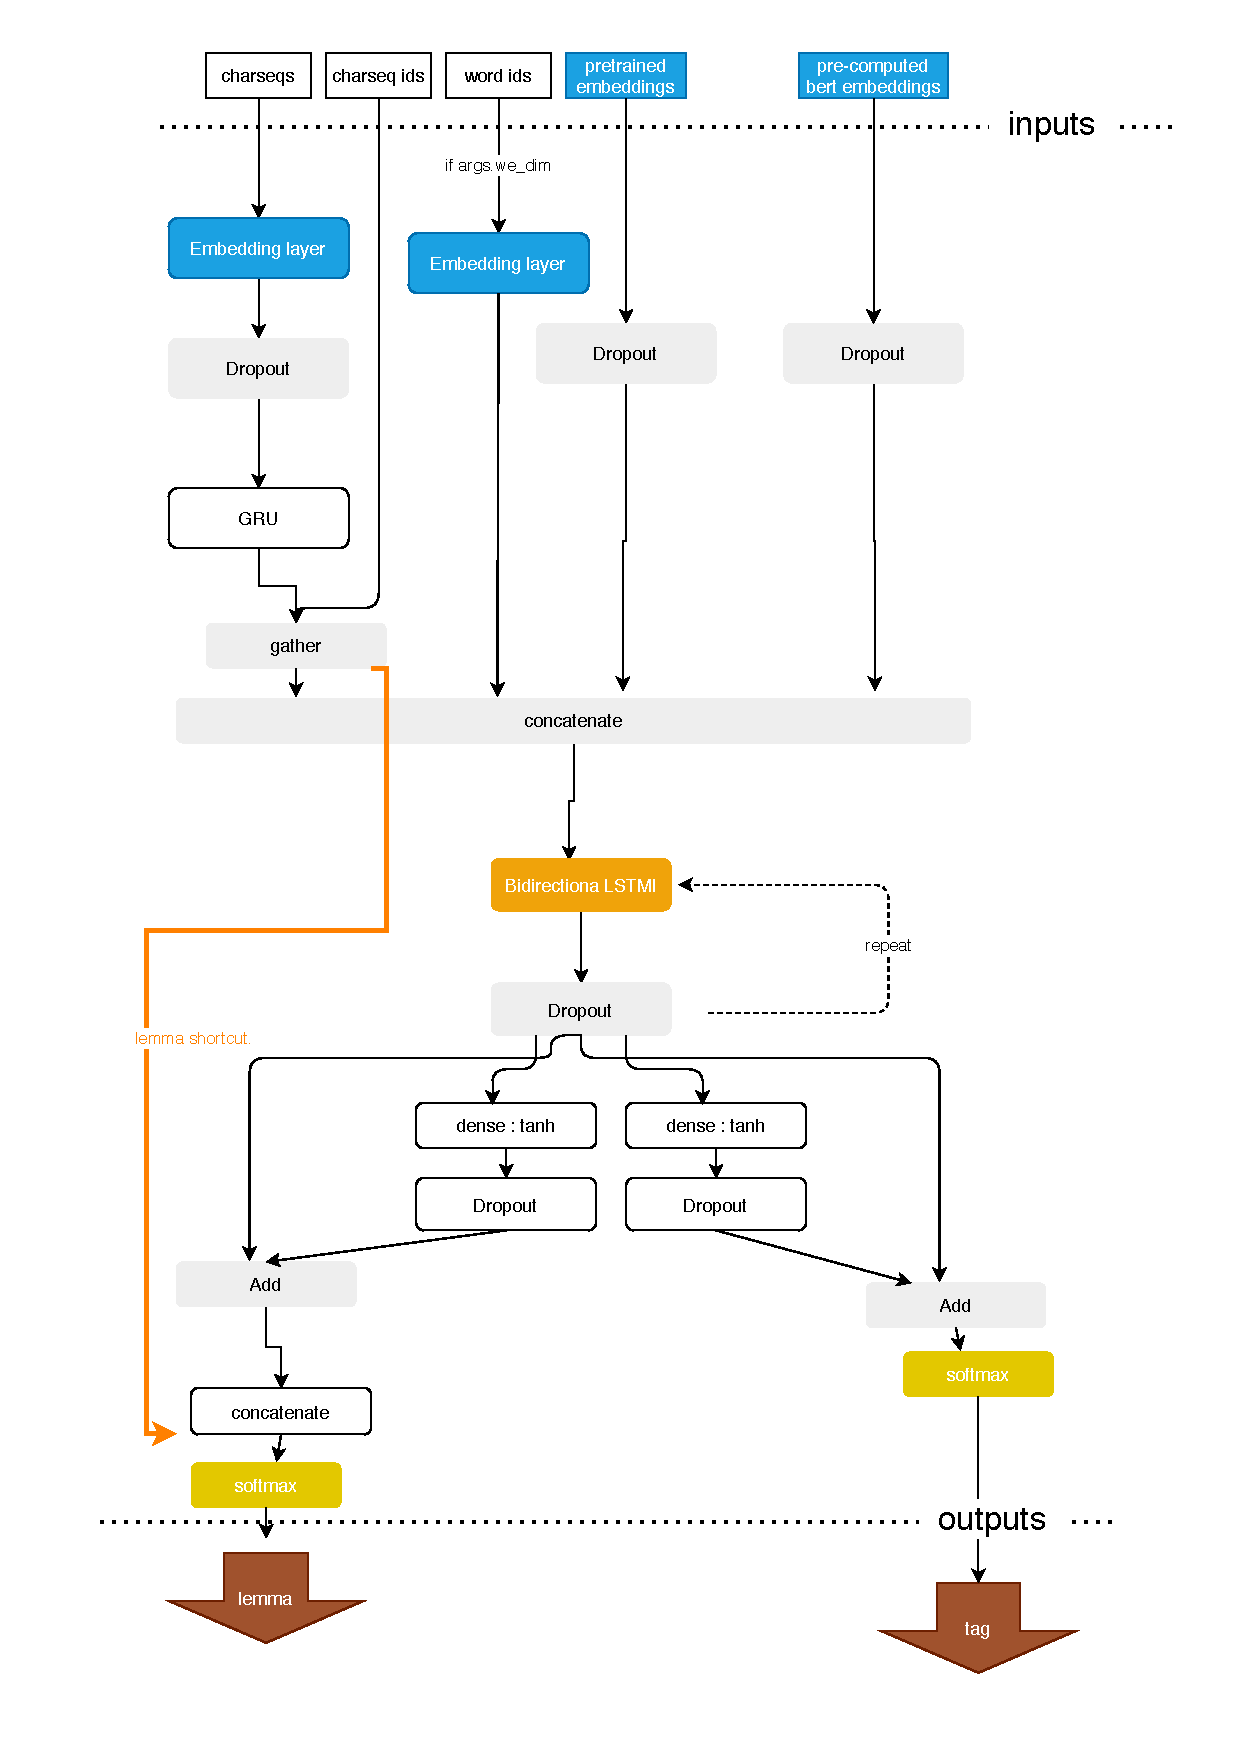
\includegraphics[width=1\columnwidth]{../img/taggermodel.pdf}
\protect\caption{Tagging and lemmatization joint model architecture.}
\label{pic:lt_arch}
\end{figure}
%TODO kolik je tech lstm a tak,vsechny dimenze (do tabulky)

%For POS tagging, we applied a straightforward model in the lines of Ling et al. (2015) – first rep- resenting each word with its embedding, contextu- alizing them with bidirectional RNNs (Graves and Schmidhuber, 2005), and finally using a softmax classifier to predict the tags. z UDpipe2

The model for lemmatization and tagging is build upon a model (and a code) for previous work on Czech NLP processing with contextual embedding \citep{Straka2019}. 
Data preprocessing is taken over from the paper as well as the structure of the lemmatizer and the tagger network, which is extended by BERT-like models, hoping for improvements. %TODO k tomu nemam citaci
Previous work showed that training tagging and lemmatization together in one network can be mutually advantageous, so both of these analyses are an output of one network, and are trained jointly. Detailed visualisation of network architecture can be found in figure \ref{pic:lt_arch}. \par The architecture of the network can be divided into three parts -- inputs, optional \acrshort{rnn}s, classification head:
\paragraph{Inputs}
An input set of the network consists of five different input types -- characters (charseqs), words (charseq ids), correct responses (word ids), pretrained embeddings, and possibly precomputed BERT embeddings (depending on the experiment type). Two other types of embeddings are created before the further processing of inputs by \acrshort{rnn} cells: character-level embeddings and another word embeddings that are, in contrast to BERT and pretrained embeddings, also trained during the training process.

\paragraph{RNN cells}
Character-level embeddings are further processed via 1 layer of \acrfull{gru} and all inputs (or their embeddings) are processed by recurrent part of network (specifically by three layers of \acrfull{lstm} cells).

\paragraph{Classification head(s)}
After the processing by recurrent neural networks, network employs two separate classification heads, one for tagging and another for lemmatization. Both heads use dense layer with tanh activation function to allow task-specific non-linear transformation as used in \citep{Straka2018} and a softmax function for obtaining the probability distribution over target classes. Lemmatization, however, presents another change -- addition of character level data without RNN processing, that are used together with the rest of the values as an input into the softmax following \citep{Straka2018}, as it leads to better performance of lemmatization in the case of shared network between both tasks.

%TODO kondraytuk bere predikci k prvnímu subwordu, jak to delam ja? 


\paragraph{Morphological Dictionary} All classification can be done with or without use of a morphological dictionary MorfFlex \citep{11234/1-1834}, that can provide possible pairs \textit{tag-lemma}. If used, the generated tag and lemma is a pair with maximal likelihood, but chosen just from the dictionary. This leads to more consistent results. 

%TODO maximal probability



%TODO nekde mam taky dropouts! zminit
\subsubsection{Experiments}
This part uses all main \textbf{experiment types} as decribed in \ref{sec:expe}: \textit{base, ls, embed, fine, simple}, and \textit{full}. Three \textbf{BERT-like models} are used for experiment setup:
\begin{itemize}
\item multilingual BERT (mBERT) \citep{Devlin2019}, 
\item XLM-RoBERTa \citep{Conneau2019}, 
\item RobeCzech \citep{Straka2021}.
\end{itemize}
XLM-RoBERTa and mBERT are trained on 100/104 different languages including Czech. RobeCzech is a recently published version of RoBERTa, trained only on Czech data. XLM-RobERTa is used only for embedding and one version of fine-tuning, and this model was omitted in other experiements because of weak results and high computational complexity. There exists another monolingual Czech model, Czert \citep{Sido2021}, which uses the original BERT architecture and was outperformed by RobeCzech \citep{Straka2021}. \par
A selection of layers is made in both ways -- last four layers (\textit{four)} and learning of weighted sum of all layers (\textit{att}). The layer attention is made only for the fine-tuning setup, and as the weighted sum does not show a significant benefit, mean of the last four layer is the only method used for other experiments.
 \par Learning rate is used as usual for each type of task and three different learning rate schedules were applied in each combination of hyperparameters: cosine decay \textit{(cos)}, inverted square root decay \textit{(isrd)} and a one epoch warm-up followed by a constant learning rate \textit{(warmup)} inspired by \citep{Kondratyuk2019} and \citep{Ruder2018}. For \textit{embed} experiments, \textit{warmup} is replaced by  a simple division of training into two parts with different learning rates. 
 
 \begin{table}[!h]
 \centering
\begin{tabular}{|l||l|}
\hline
hyperparametr   & \multicolumn{1}{l|}{value} \\ \hline \hline
beta\_2          & 0.99                       \\ \hline
optimizer       & Adam                       \\ \hline
cle\_dim         & 256                        \\ \hline
dropout         & 0.5                        \\ \hline
label smoothing & 0.3                        \\ \hline
rnn\_cell        & LSTM                       \\ \hline
rnn\_cell\_dim    & 512                        \\ \hline
rnn\_layers      & 3                          \\ \hline
we\_dim          & 512                        \\ \hline
word\_dropout    & 0.2                        \\ \hline
batch size & 64 \\ \hline
\end{tabular}
\caption[Hyperparameters of tagging and lemmatization common to all experiments]{Hyperparameters of tagging and lemmatization common to all experiments (if they make sense in the context of experiments).}
\label{tab:hyp_all}
\end{table}
Batches have size 64, given by the compromise between the pursuit of relatively big batch size and computational resources. Summary of hyperparameters, which do not differ across experiments is presented in table \ref{tab:hyp_all}. Other hyperparameters for each experiment are in table \ref{att:1}.
\par 
Reimplementation of \citep{Straka2019a} without any BERT-like model incorporation serves as a baseline.

\subsection{Results and Discussion}
Best presented model (experiment no. 18) achieved the same or better results than the current \acrlong{sota} tagging and lemmatization results (table \ref{tab:all_prew}). Complete results are in table \ref{tab:all_res_tl}. Experiment \textit{tl\_18} is the version with fine-tuning, Czech monolingual model, RobeCzech, and without layer attention, although the difference from comparable experiment with layer attention is insignificant and can be just accidental. The dominance of the Czech model was expected and additional expert knowledge contained in the complicated architecture was also assumed to be better. Experiments also showed that fine-tuning approach achieves better results than full training from the beginning. This may be due to the choice of hyperparameters, especially the learning rate, but the standard ones were selected, implying that at best, it is more difficult to find the right parameters for\textit{full} and \textit{simple} variants. Although \textit{simple} experiments presents standard approach of using pretrained BERT models, they turned out being less successful even than \textit{embed} experiments, that are faster to train and less memory intensive. 

\begin{table}[!h]
\centering
  \resizebox{\columnwidth}{!}{\begin{tabular}{|l||ccc||ccc|}
  \hline
\multirow{2}{*}{Experiment} & \multicolumn{3}{c||}{Without Dictionary}  &
      \multicolumn{3}{c|}{With Dictionary} \\ 
    & Tags & Lemmas & Both & Tags & Lemmas & Both \\ \hline \hline
    \textit{\citep{Straka2019}} & \textit{97.94} & \textit{98.75} & \textit{97.31} & \textit{98.05} & \textit{98.98} & \textit{97.65 }\\ \hline
   \textit{ StrakaC} & \textit{97.67} & \textit{98.63} & \textit{97.02} & \textit{97.91 }& \textit{98.94} & \textit{97.51} \\ \hline
     \textit{RobeCzech} & \textit{98.43} & \textit{98.79}  & \textit{97.83}  & \textit{98.50} & \textit{\textbf{99.00}}  & \textit{98.11} \\ \hline \hline
      baseline & 97.04  & 98.56  & 96.41 &  97.31   & 98.83  & 96.90 \\ \hline 
    emb(12) & 98.38  &98.79  & 97.80 & 98.48  & 98.99 & 98.10 \\ \hline
    best(18) & \textbf{98.50}  & \textbf{98.80} &\textbf{ 97.90}  & \textbf{98.57}  & \textbf{99.00}  & \textbf{98.19}  \\ \hline  
  \end{tabular}}
  \caption[Comparison of our best results and previous work]{
  \textit{Straka2019C} is a comparable solution  (BERT embeddings only) from \citep{Straka2019} to \textit{emb}, which was transformed into Tensorflow 2 in this work as a \textit{baseline}. \textit{Emb} is a solution with static BERT embeddings and \textit{best(18) is the best resulting model in this thesis (experiment id = 18). }}
\label{tab:all_prew} 
\end{table}


%TODO vsechny Figure a table se stejnym pismenem

\begin{table}[!h]
\resizebox{\columnwidth}{!}{
\begin{tabular}{|l|l|l|l|l|l||llllll|}
\hline
\multicolumn{2}{|c|}{\multirow{2}{*}{Model}} &
  \multirow{2}{*}{EXPE} &
  \multirow{2}{*}{EP} &
  \multirow{2}{*}{LAYERS} &
  \multirow{2}{*}{LR} &
  \multicolumn{2}{c}{Lemmas} &
  \multicolumn{2}{c}{Tags} &
  \multicolumn{2}{c|}{Both} \\
\multicolumn{2}{|l|}{} &  &  &  &  & Raw & Dict & Raw & Dict & Raw & Dict  \\ \hline \hline
0  & NA                           & base                    & A	& NA               & simple & 98.58  & 98.81   & 97.05   & 97.31    & 96.43     & 96.9       \\ \hline
1  & NA                           & ls                      & B	& NA               & simple & 98.55  & 98.81   & 97.12   & 97.34    & 96.51     & 96.94      \\ \hline
2  & \multirow{3}{*}{mBERT}       & \multirow{9}{*}{embed}  & B	& four             & simple & 98.69  & 98.93   & 97.83   & 97.98    & 97.17     & 97.58      \\ \cline{1-1} \cline{4-12}
3  &                              &                         & C	& four                     & cos    & 98.74  & 98.95   & 97.91   & 98.04    & 97.28     & 97.63      \\ \cline{1-1} \cline{4-12}
4  &                              &                         & C	& four                     & isrd   & 98.73  & 98.94   & 97.89   & 98.02    & 97.28     & 97.61      \\ \cline{1-2} \cline{4-12}
5  & \multirow{3}{*}{xlm-Roberta} &                         & B	& four             & simple & 98.57  & 98.8    & 97.33   & 97.54    & 96.68     & 97.12      \\ \cline{1-1} \cline{4-12}
6  &                              &                         & C	& four                     & cos    & 98.6   & 98.83   & 97.45   & 97.62    & 96.81     & 97.21      \\ \cline{1-1} \cline{4-12}
7  &                              &                         & C	& four                     & isrd   & 98.59  & 98.83   & 97.44   & 97.61    & 96.81     & 97.2       \\ \cline{1-2} \cline{4-12}
8  & \multirow{3}{*}{RoBECzech}   &                         & B	& four             & simple & 98.77  & 98.97   & 98.38   & 98.48    & 97.78     & 98.08      \\ \cline{1-1} \cline{4-12}
9  &                              &                         & C	& four                     & cos    & 98.79  & 98.99   & 98.38   & 98.48    & 97.80      & 98.10      \\ \cline{1-1} \cline{4-12}
10 &                              &                         & C	& four                     & isrd   & 98.78  & 98.98   & 98.4    & 98.48    & 97.8      & 98.09      \\ \hline
11 & \multirow{3}{*}{mBERT} & \multirow{9}{*}{fine}         & D	& four     & simple & 98.69 & 98.93 & 97.84 & 97.99 & 97.21 & 97.59 \\ \cline{1-1} \cline{4-12}
12 &                              &                         & E	& four             & cos    & 98.72  & 98.95   & 97.97   & 98.08    & 97.33     & 97.68      \\ \cline{1-1} \cline{4-12}
13 &                              &                         & E	& four             & isrd   & 98.68  & 98.9    & 97.72   & 97.86    & 97.09     & 97.46      \\ \cline{1-2} \cline{4-12}
14 & \multirow{3}{*}{xlm-Roberta} &                         & D	& four     & simple & 98.62  & 98.84   & 97.72   & 97.9     & 97.07     & 97.48      \\ \cline{1-1} \cline{4-12}
15 &                              &                         & E	& four             & cos    & 98.67  & 98.9    & 97.95   & 98.09    & 97.32     & 97.69      \\ \cline{1-1} \cline{4-12}
16 &                              &                         & E	& four             & isrd   & 98.63  & 98.85   & 97.66   & 97.83    & 97.03     & 97.41      \\ \cline{1-2} \cline{4-12}
17 & \multirow{3}{*}{RoBECzech}   &                         & D	& four     & simple & 98.78  & 98.98   & 98.46   & 98.55    & 97.86     & 98.16      \\ \cline{1-1} \cline{4-12}
18 &                              &                         & E	& four             & cos    & \textbf{98.80}   & \textbf{99.00 }     & \textbf{98.50}    & \textbf{98.57}    & \textbf{97.90 }     & \textbf{98.19 }     \\ \cline{1-1} \cline{4-12}
19 &                              &                         & E	& four             & isrd   & 98.76  & 98.95   & 98.33   & 98.41    & 97.72     & 98.02      \\ \cline{1-2} \cline{4-12} \hline
20 & \multirow{3}{*}{mBERT}  &  \multirow{9}{*}{fine att}   & D	& att                       & simple & 98.67  & 98.91   & 97.76   & 97.92    & 97.13     & 97.52      \\ \cline{1-1} \cline{4-12}
21 &                              &                         & E	& att              & cos    & 98.72  & 98.95   & 97.98   & 98.1     & 97.34     & 97.69      \\ \cline{1-1} \cline{4-12}
22 &                              &                         & E	& att              & isrd   & 98.67  & 98.91   & 97.69   & 97.85    & 97.05     & 97.45      \\ \cline{1-2} \cline{4-12}
23 & \multirow{3}{*}{xlm-Roberta} &                         & D	& att      & simple & 98.6   & 98.81   & 97.62   & 97.77    & 96.96     & 97.35      \\ \cline{1-1} \cline{4-12}
24 &                              &                         & E	& att              & cos    & 98.67  & 98.89   & 97.91   & 98.06    & 97.29     & 97.66      \\ \cline{1-1} \cline{4-12}
25 &                              &                         & E	& att              & isrd   & 98.65  & 98.86   & 97.65   & 97.81    & 97.03     & 97.41      \\ \cline{1-2} \cline{4-12}
26 & \multirow{3}{*}{RoBECzech}   &                         & D	& att      & simple & 98.77  & 98.97   & 98.38   & 98.47    & 97.79     & 98.08      \\ \cline{1-1} \cline{4-12}
27 &                              &                         & E	& att              & cos    & \textbf{98.8}   & 98.99   & 98.47   & 98.54    & 97.88     & 98.16      \\ \cline{1-1} \cline{4-12}
28 &                              &                         & E	& att              & isrd   & 98.77  & 98.96   & 98.33   & 98.41    & 97.72     & 98.01      \\ \hline
29 & \multirow{3}{*}{mBERT}       & \multirow{9}{*}{simple} & F	& four                     & warmup & 98.17  &         & 97.32   &          & 96.46     &            \\ \cline{1-1} \cline{4-12}
30 &                              &                         & G	& four                     & cos    & 98.15  &         & 97.39   &          & 96.47     &            \\ \cline{1-1} \cline{4-12}
31 &                              &                         & G	& four                     & isrd   & 98.13  &         & 97.12   &          & 96.29     &            \\ \cline{1-2} \cline{4-12}
35 & \multirow{3}{*}{RoBECzech}   &                         & F	& four                     & warmup & 98.49  &         & 98.28   &          & 97.41     &            \\ \cline{1-1} \cline{4-12}
36 &                              &                         & G	& four                     & cos    & 98.46  &         & 98.30   &          & 97.39     &            \\ \cline{1-1} \cline{4-12}
37 &                              &                         & G	& four                     & isrd   & 98.59  &         & 98.27   &          & 97.53     &            \\ \hline
38 & \multirow{3}{*}{mBERT}       & \multirow{9}{*}{full}   & F	& four                     & warmup & 98.16  & 98.86   & 97.35   & 97.79    & 96.46     & 97.34      \\ \cline{1-1} \cline{4-12}
39 &                              &                         & G	& four                     & cos    & 98.04  & 98.85   & 97.36   & 97.81    & 96.3      & 97.34      \\ \cline{1-1} \cline{4-12}
40 &                              &                         & G	& four                     & isrd   & 98.22  & 98.86   & 97.34   & 97.73    & 96.46     & 97.29      \\ \cline{1-2} \cline{4-12}
44 & \multirow{3}{*}{RoBECzech}   &                         & G	& four                     & warmup & 98.49  & 98.95   & 98.21   & 98.34    & 97.38     & 97.93      \\ \cline{1-1} \cline{4-12}
45 &                              &                         & G	& four                     & cos    & 98.25  & 98.95   & 98.17   & 98.33    & 97.08     & 97.89      \\ \cline{1-1} \cline{4-12}
46 &                              &                         & G	& four                     & isrd   & 98.55  & 98.99   & 98.19   & 98.35    & 97.39     & 97.95      \\ \hline

\end{tabular}
}
\caption[Complete results for tagging and lemmatization]{This table presents complete results for tagging and lemmatizationt tasks. Column EP presents number of epochs and corresponding learning rates are explained in Attachement \protect\ref{att:1} }
\label{tab:all_res_tl}
\end{table}

\subsubsection{Error Analysis}
%TODO sjednotit názvy modelů
This section offers a little exploration of differences in error across models. This comparison includes three models: 
\begin{itemize}
\item tl\_18 -- the best model in tagging and lemmatization,
\item tl\_3 -- the best model with mBERT,
\item tl\_1 -- the baseline model with label smoothing.
\end{itemize} 

\paragraph{best vs. baseline}
The best model (tl\_18) improves prediction in $3,247$ tags and is worse in 421 tag predictions. More than 80\% of newly correctly predicted tags are composed by three parts of speech: NN (noun), AA (adjective), and RR (preposition). Table \ref{att:tags1} presents improved tags with a frequency at least 10. The most frequent tag ( \texttt{NNIS1-----A----}) presents proper names of places (e.g. Jersey, Tenesee), but we can see that other frequent tags are nominatives and accusatives of masculinum, singular,  inainamate (cs: \textit{rod mužský neživotný}) or femininum, plural. These two cases have the same form for mentioned categories, so they are indistinguishable without context, and that is where BERT showed to be very useful. The same situation is with adjectives, again mostly nominative or accusative of the same form, for example words \textit{další} (following) or \textit{stínový} (shadowy). The third category are prepositions that can be connected with both accusative and dative as \textit{na} (on), or \textit{o} (about).

%TODO kolik lemmata

\paragraph{mBERT vs. RobeCzech}
Best mBERT is better in 468 tags and worse in $1,703$ tags than the best model. The most frequent tags improved by \textit{tl\_18} are similar to previous comparison. Nominative and accusative are again the most common cases improved, but the differences between these two models are not so significant. This results in verbs appearing higher in the table of most frequent tags, although the absolute value of better predictions on verbs is similar to previous comparison. In both situations, improved verbs predictions relate mostly to verbs with the same form in singular and plural of the third-person, e.g. \textit{vyváží} (exports) or \textit{stojí} (stands). The complete table of the most frequent tags is available in table \ref{att:tags2}.
%TODO kolik lemmata
%TODO je v necem mBERT lepsi?

%\section{Sentiment Analysis}
\label{chap:sent}
As stated in \citep{Veselovska}: "Sentiment analysis, also known as opinion mining, is an automatic detection of a positive or negative polarity, or neutrality of ... a text sequence", which is exactly as the sentiment analysis is understood in this work, although there are some other definitions consisting of e.g. opinion extraction, irony or stance \citep{Montoyo2012}. Another tasks related to sentiment analysis is a subjectivity analysis (whether the presented opinion is objective or highly subjective), which is also not included in this work, mainly because the lack of labelled data for Czech. It is possible to analyze individual expressions, sentences or whole documents \citep{Veselovska} and this work focuses on the document level classification.
\subsection{Task definition}
\paragraph{Sentiment analysis} \mbox{}\\
\textit{input:} sequence of sentences (a whole post or comment, depending on the source) \\
\textit{output:} prevailing sentiment of the input from categories: neutral, positive, negative.
\par

\paragraph{Metric} For evaluating performance, two metrics are used: macro-averaged F1 score and accuracy. Both metrics are chosen for better comparability with previous work.

\subsection{Related Work}
citace:
\citep{Cano2019}
\citep{Kittask2020} .. estonian
\citep{Lenc2016} sentiment in czech
\citep{Hercig2018}
\citep{Li}
\citep{Libovicky} presents state-of-the art results in three czech NLP tasks including sentiment analysis. They use only CSFD dataset with resulting accuracy 80.8 .1 which is still not so good as Brychcín (81.5.3). The second mentioned paper, however, uses quite complicated method for classification incorporating the fact of which movie is reviewed. 

Bachelor thesis which aplies bert on sentiment analysis in czech:
%https://dspace.cvut.cz/bitstream/handle/10467/83127/F8-BP-2019-Langr-Lukas-thesis.pdf?sequence=-1&isAllowed=y
results are accuracy 84 with tfidf and about 81 with bert and they used mall dataset.

\subsection{Dataset and Preprocessing}
%TODO zjistit jaka jsou na to porovnavaci data This work primary tries to improve existing tasks and show the ability of contextualized embeddings to improve results, so tasks with existing data and results were selected.  %TODO why?
Four main Czech datasets with sentiment annotation are available: user reviews from MALL.cz (mall), film reviews from csfd.cz (csfd), news from Aktualne.cz (aktualne) and posts from czech branch pages on facebook.cz (facebook). As \textit{aktualne} dataset turned out to be problematical because the text were ambiguous even for annotators, and its authors later used other mentioned datasets \citep{Veselovska}, this work also focuses only on the three other data sources -- \textit{mall}, \textit{csfd} and \textit{facebook} \footnote{All three datasets are all available here: http://liks.fav.zcu.cz/sentiment/}. Some experiment are also performed with in-domain training on Eglish data. For this purpose is used \textit{imdb} dataset \footnote{https://www.tensorflow.org/datasets/catalog/imdb\_reviews}, which contains movie review from the biggest movie rating website imdb.com. This leads to some problems described later in this section, because English dataset contains only binary classification (positive/negative). Table \ref{tab:datasets} summarize each dataset.
%TODO popis tabulky
\begin{center}
\begin{table}[]
\begin{tabular}{|l||lll|}
\hline
     & length & labels                                                                & domain        \\ \hline \hline
\textbf{mall}     & 145306 & \begin{tabular}[c]{@{}l@{}}positive\\ neutral\\ negative\end{tabular} & domestic appliance reviews                             \\ \hline
\textbf{csfd} & 91304  & \begin{tabular}[c]{@{}l@{}}positive\\ neutral\\ negative\end{tabular} & movie reviews \\ \hline
\textbf{facebook} & 9752   & \begin{tabular}[c]{@{}l@{}}positive\\ neutral\\ negative\end{tabular} & \begin{tabular}[c]{@{}l@{}}brand pages of e.g. shops or mobile networks \\ providers\end{tabular} \\ \hline
\textbf{imdb} & 25000  & \begin{tabular}[c]{@{}l@{}}positive\\ negative\end{tabular}           & movie reviews \\ \hline
\end{tabular}
\label{tab:datasets}
\caption{Three Czech datasets (mall, facebook, csfd) and one English (imdb) are used for training in this work.}
\end{table}
\end{center}


%TODO je to rozdleeno se stratifikací?
%TODO popis obrazku
\begin{figure}[!ht]
\centering
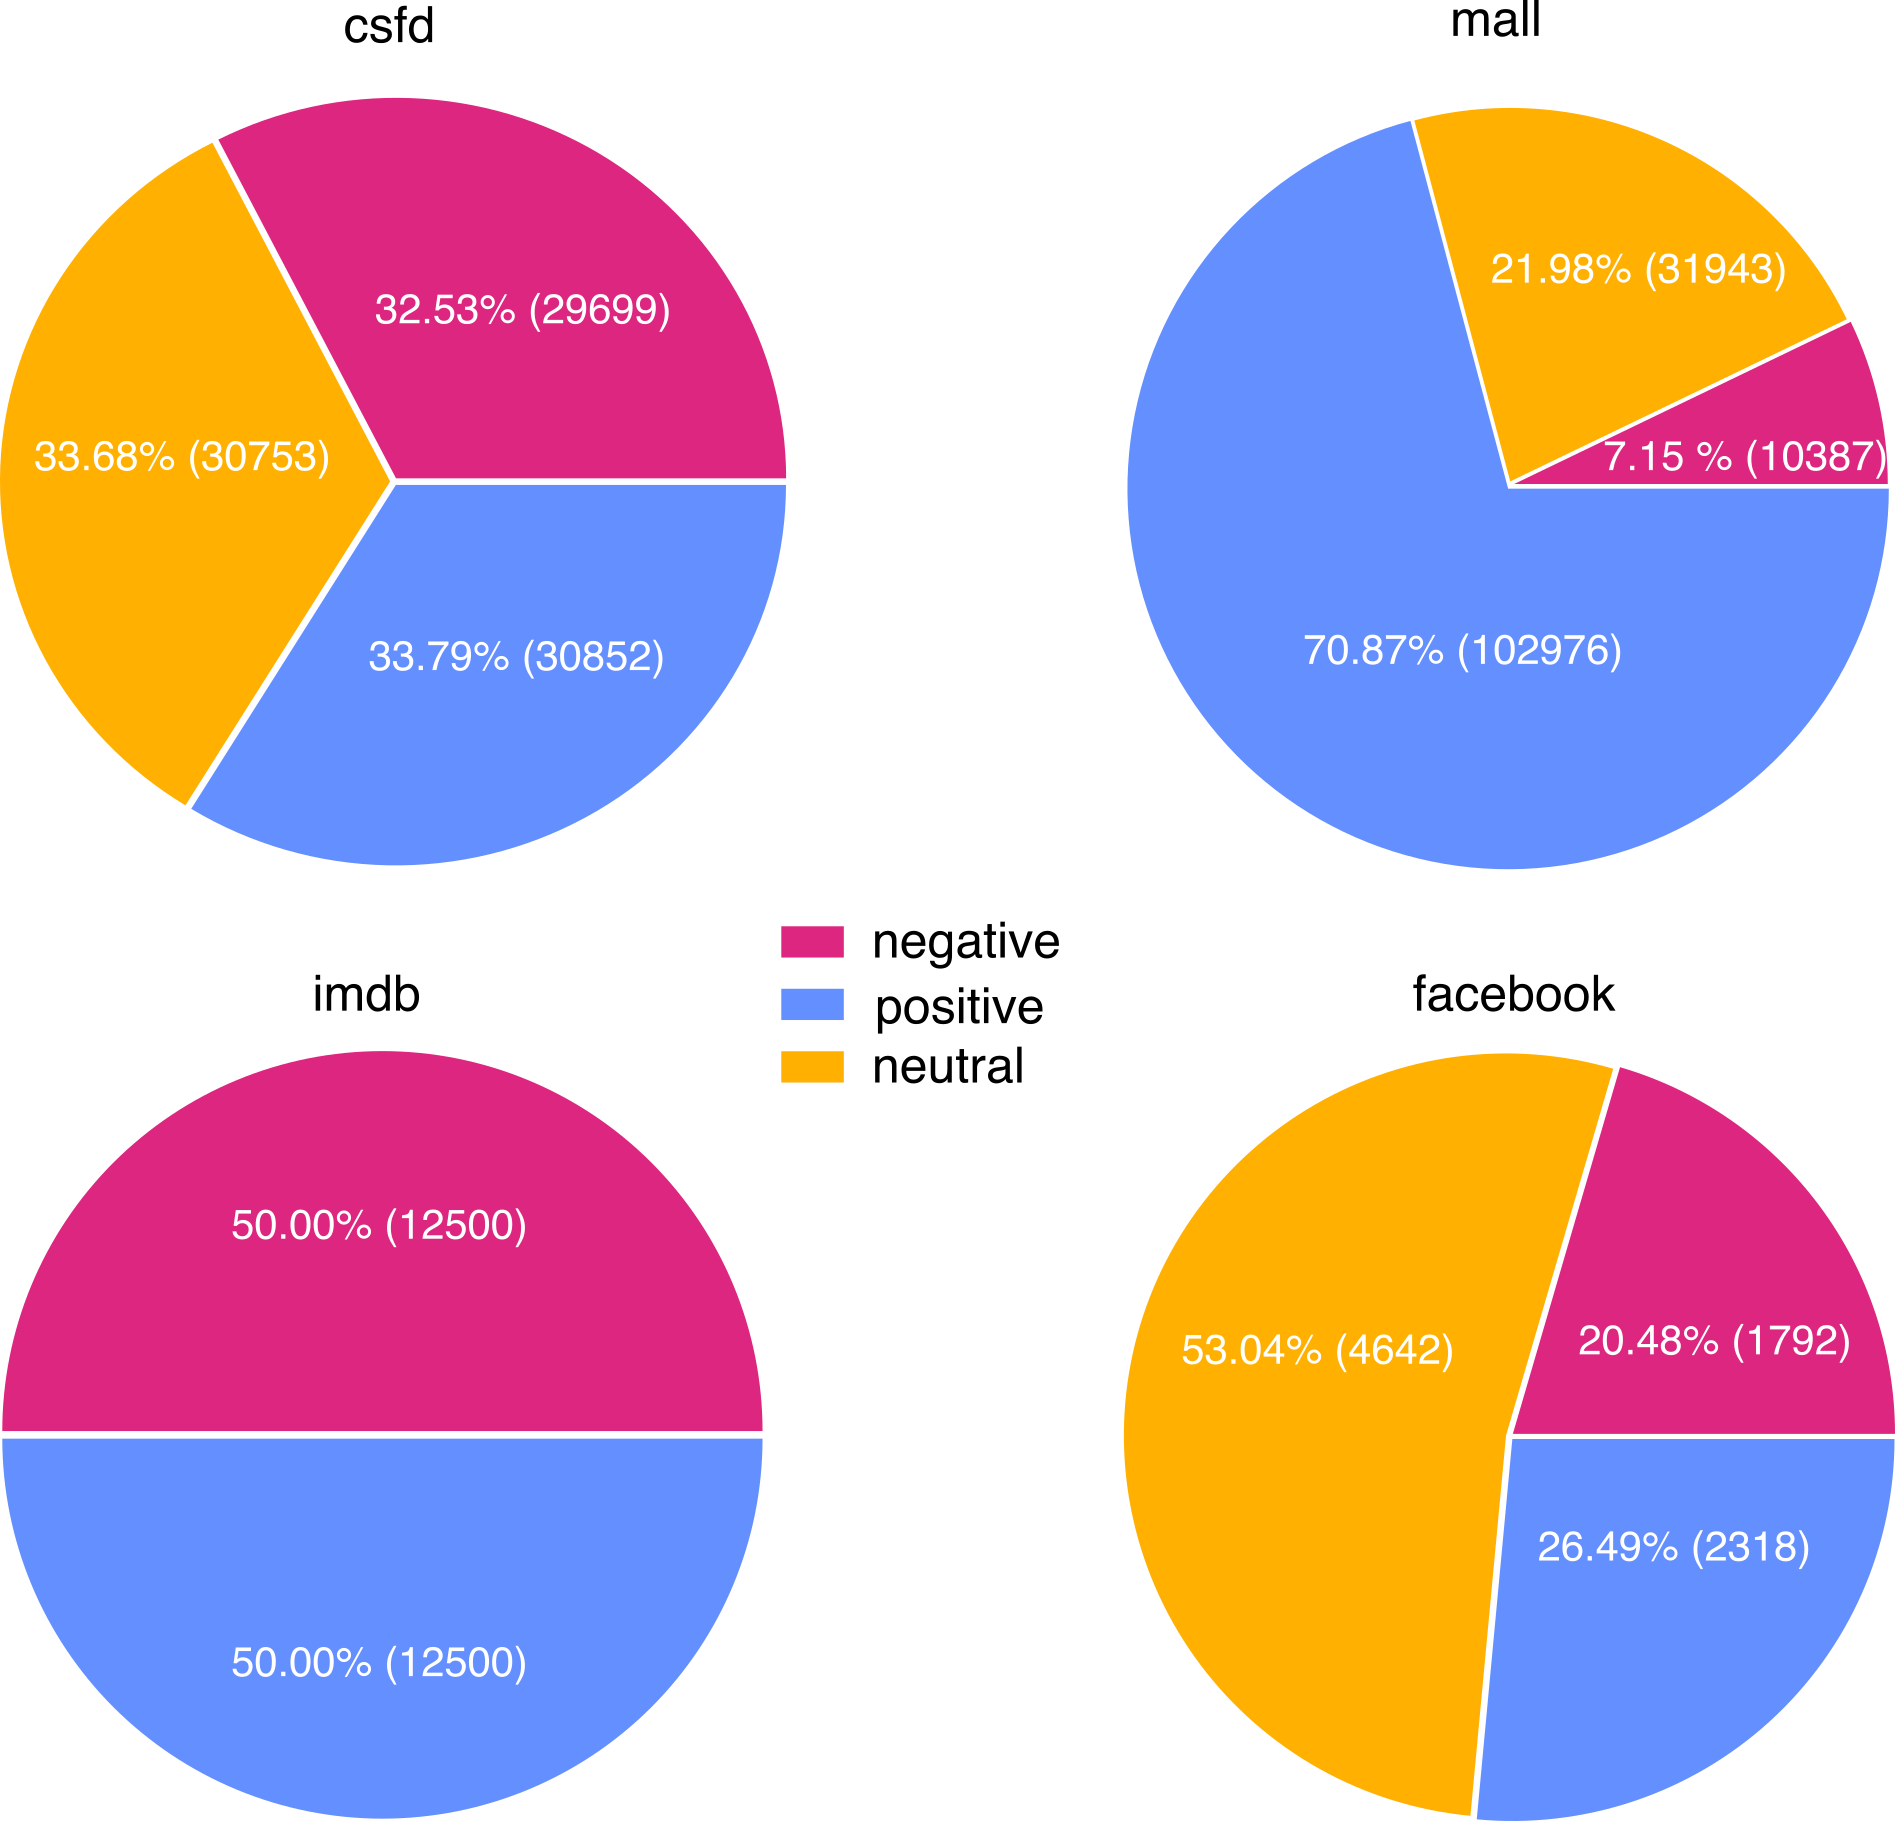
\includegraphics[width=1\columnwidth]{../img/dist_all.png}
\protect\caption{Distribution of positive/neutral/negative labels in each dataset.}
\label{pic:dist}
\end{figure}

As can be seen in figure \ref{pic:dist}
distribution of labels differs among datasets. Moreover, Figure \ref{pic:dist_all}
\begin{figure}[!ht]
\centering
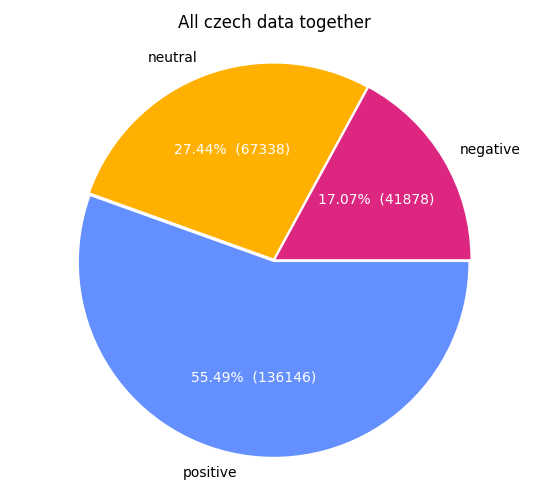
\includegraphics[width=0.7\columnwidth]{../img/all.png}
\protect\caption{Percentage and absolute values of labels in all three Czech datasets together.}
\label{pic:dist_all}
\end{figure}
%TODO all má blbý nadpis
shows, that the resulting dataset is highly unbalanced, which causes divergence and stuck in training. Due to the big part of labels being positive, many learning strategies just ended with predicting only \textit{positive} class, i.e. 55\% accuracy, so unfortunately learned nothing. 

%This was the the case for following experiments settings:
%learning rate of $2e-3$ for 10 epochs. This ended with predicting only one class (positive). Some progress showed the followign approach:"2:5e-5,1:2e-5, unfreezed" for facebook data only (which are balanced). This results are above 71 for accuracy (Test accuracy: 0.726
%F1 metrics: 0.7077061630227595 weighted).


\subsection{Experiments and Architecture}
The main division of experiments is by the input dataset -- each of Czech models separately and one joint dataset consisting of all Czech datasets, i.e. four different datasets. All variants performed both layers attention and an average of last four layers. As for the learning rate, all experiments were made with learning rate $3 \times 10^{-5}$ and there were always two types of learning rate decay -- cosine and inverse square root decay. 
\par
Network architecture is much simpler than in tagging and lemmatization task and corresponds to \textit{simple} setting of these tasks -- only BERT-like model and classification head consisting of layer with softmax activation function. %TODO a neni tam nahodou jeste neco?

\begin{figure}[h]
\centering
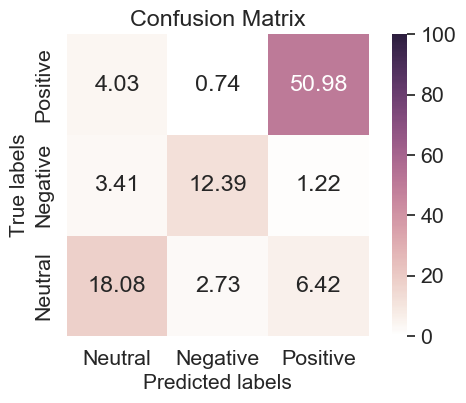
\includegraphics[width=1\columnwidth]{../img/confusion_matrix}
\protect\caption{Normalized confusion matrix}
\label{pic:conf1}
\end{figure}

\subsection{Results and Discussion}
%I tried another approach:
%Because the facebook dataset is balanced, I pretrained the model first on facebook and after reaching a decent accuracy, i further trained the model on the join data:
%for ten epochs with learning rate 5e-5 and an effecctive batch size 48.
%[[ 6240 914 2783]
%[ 1236 4447 529]
%[ 1050 273 19020]]
%Test accuracy: 0.814068837005371
%F1 metrics: 0.8087903170140932

%The pretraining model was obtained as:
%without freezing, batch size 48, 2:5e-5,4:2e-5



%Than I trained for 3 more epochs:
%[[ 6599 995 2343]
%[ 1246 4520 446]
%[ 1470 269 18604]]
%Test accuracy: 0.8145072892688808
%F1 metrics: 0.8119431050948791
%TODO  \ref{pic:conf1}

Baseline for this task is tf-idf method %TODO nekde je popsana v prni kapitole
, which resulted in 
[[ 4310   102  3015]
 [  685  1016   779]
 [  842    48 20227]]
              precision    recall  f1-score   support

           0       0.74      0.58      0.65      7427
           1       0.87      0.41      0.56      2480
           2       0.84      0.96      0.90     21117

    accuracy                           0.82     31024
   macro avg       0.82      0.65      0.70     31024
weighted avg       0.82      0.82      0.81     31024


% Please add the following required packages to your document preamble:
% \usepackage{multirow}
\begin{table}[]
\resizebox*{!}{\textheight}{\begin{tabular}{|l|l|l|l||ll|}
\hline
\multicolumn{2}{|l|}{MODEL}       & EXPE                      & LRTYPE                & Acc    & F1   \\ \hline  \hline
1  & \multirow{6}{*}{mBERT}     & czech                     & \multirow{3}{*}{Isrd} & 0,81   & 0,81 \\ \cline{1-1} \cline{3-3} \cline{5-6} 
2  &                            & zero                      &                       & 0,50   & 0,45 \\ \cline{1-1} \cline{3-3} \cline{5-6} 
3  &                            & eng                       &                       & 0,81   & 0,81 \\ \cline{1-1} \cline{3-6} 
4  &                            & czech                     & \multirow{3}{*}{cos}  & 0,83   & 0,82 \\ \cline{1-1} \cline{3-3} \cline{5-6} 
5  &                            & zero                      &                       & 0,53   & 0,48 \\ \cline{1-1} \cline{3-3} \cline{5-6} 
6  &                            & eng                       &                       & 0,83   & 0,82 \\ \hline
13 & \multirow{4}{*}{RoBECzech} & czech                     & \multirow{2}{*}{isrd} & 0,81   & 0,81 \\ \cline{1-1} \cline{3-3} \cline{5-6} 
14 &                            & zero                      &                       & 0,55   & 0,48 \\ \cline{1-1} \cline{3-6} 
16 &                            & czech                     & \multirow{2}{*}{cos}  & 0,84   & 0,84 \\ \cline{1-1} \cline{3-3} \cline{5-6} 
17 &                            & zero                      &                       & 0,58   & 0,49 \\ \hline
19 & \multirow{6}{*}{mBERT}     & czech                     & \multirow{3}{*}{Isrd} & 0,82   & 0,81 \\ \cline{1-1} \cline{3-3} \cline{5-6} 
20 &                            & zero                      &                       & 0,54   & 0,48 \\ \cline{1-1} \cline{3-3} \cline{5-6} 
21 &                            & eng                       &                       & 0,82   & 0,81 \\ \cline{1-1} \cline{3-6} 
22 &                            & czech                     & \multirow{3}{*}{cos}  & 0,83   & 0,82 \\ \cline{1-1} \cline{3-3} \cline{5-6} 
23 &                            & zero                      &                       & 0,52   & 0,47 \\ \cline{1-1} \cline{3-3} \cline{5-6} 
24 &                            & eng                       &                       & 0,83   & 0,82 \\ \hline
31 & \multirow{4}{*}{RoBECzech} & czech                     & \multirow{2}{*}{isrd} & 0,83   & 0,83 \\ \cline{1-1} \cline{3-3} \cline{5-6} 
32 &                            & zero                      &                       & 0,58   & 0,50 \\ \cline{1-1} \cline{3-6} 
34 &                            & czech                     & \multirow{2}{*}{cos}  & 0,84   & 0,84 \\ \cline{1-1} \cline{3-3} \cline{5-6} 
35 &                            & zero                      &                       & 0,58   & 0,51 \\ \hline
37 & \multirow{2}{*}{mBERT}     & \multirow{7}{*}{facebook} & Isrd                  & 0,75   & 0,75 \\ \cline{1-1} \cline{4-6} 
38 &                            &                           & cos                   & 0,76   & 0,76 \\ \cline{1-2} \cline{4-6} 
41 & \multirow{5}{*}{RoBECzech} &                           & isrd                  & 0,80   & 0,80 \\ \cline{1-1} \cline{4-6} 
42 &                            &                           & simple                & 0,79   & 0,79 \\ \cline{1-1} \cline{4-6} 
43 &                            &                           & \multirow{3}{*}{cos}  & 0,82   & 0,81 \\ \cline{1-1} \cline{5-6} 
44 &                            &                           &                       & 0,81   & 0,81 \\ \cline{1-1} \cline{5-6} 
45 &                            &                           &                       & 0,82 & 0,82 \\ \hline
46 & \multirow{2}{*}{mBERT}     & \multirow{4}{*}{facebook} & Isrd                  & 0,76   & 0,76 \\ \cline{1-1} \cline{4-6} 
47 &                            &                           & cos                   & 0,77   & 0,77 \\ \cline{1-2} \cline{4-6} 
50 & \multirow{2}{*}{RoBECzech} &                           & isrd                  & 0,80   & 0,79 \\ \cline{1-1} \cline{4-6} 
51 &                            &                           & cos                   & 0,806  & 0,80 \\ \hline
52 & \multirow{2}{*}{mBERT}     & \multirow{8}{*}{mall}     & Isrd                  & 0,83   & 0,83 \\ \cline{1-1} \cline{4-6} 
53 &                            &                           & cos                   & 0,84   & 0,84 \\ \cline{1-2} \cline{4-6} 
56 & \multirow{2}{*}{RoBECzech} &                           & isrd                  & 0,83   & 0,83 \\ \cline{1-1} \cline{4-6} 
57 &                            &                           & cos                   & 0,85   & 0,84 \\ \cline{1-2} \cline{4-6} 
58 & \multirow{2}{*}{mBERT}     &                           & Isrd                  & 0,83   & 0,83 \\ \cline{1-1} \cline{4-6} 
59 &                            &                           & cos                   & 0,84   & 0,84 \\ \cline{1-2} \cline{4-6} 
62 & \multirow{2}{*}{RoBECzech} &                           & isrd                  & 0,84   & 0,84 \\ \cline{1-1} \cline{4-6} 
63 &                            &                           & cos                   & 0,85   & 0,84 \\ \hline
64 & \multirow{2}{*}{mBERT}     & \multirow{8}{*}{csfd}     & Isrd                  & 0,81   & 0,81 \\ \cline{1-1} \cline{4-6} 
65 &                            &                           & cos                   & 0,82   & 0,82 \\ \cline{1-2} \cline{4-6} 
68 & \multirow{2}{*}{RoBECzech} &                           & isrd                  & 0,83   & 0,83 \\ \cline{1-1} \cline{4-6} 
69 &                            &                           & cos                   & 0,85   & 0,85 \\ \cline{1-2} \cline{4-6} 
70 & \multirow{2}{*}{mBERT}     &                           & Isrd                  & 0,82   & 0,82 \\ \cline{1-1} \cline{4-6} 
71 &                            &                           & cos                   & 0,82   & 0,82 \\ \cline{1-2} \cline{4-6} 
74 & \multirow{2}{*}{RoBECzech} &                           & isrd                  & 0,83   & 0,83 \\ \cline{1-1} \cline{4-6} 
75 &                            &                           & cos                   & 0,84   & 0,84 \\ \hline
\end{tabular}}
\end{table}



%Because BERT model was trained on multilingual data, it is naturally not so good in language minoritly presented in the Bert's training data. When transfering the learned knowledge to czech sentiment task, we actually want to improve model in two ways: teach it something more specific about given task, i.e., sentiment, and improve its knowledge about selected language (czech in this case). By using czech sentiment dataset, both thing are incorporated into training. To obtained better results and following the \citep{Putra}, I also selected english sentiment dataset. The idea behind is that BERT is quite good in english and maybe can learn faster useful knowledge about the given task from data in more familiar language.















\chapter{Implementation analysis}
\label{chap:impl}
The main purpose of this chapter is to offer the technical description of the code accompanying this work for better reproducibility and possible further experiments on every of presented tasks. This chapter describes an implementation of all language models, other related code and also presents all used libraries and technologies.
% and this chapter is concluded with a presentation of experiment types common for training of both tasks presented in following chapters.
\par
All code forms an attachment of this work and is also publicly available in GitHub \footnote{https://github.com/flower-go/DiplomaThesis}. Experiment were performed on Artificial Intelligence Cluster (AIC) \footnote{https://aic.ufal.mff.cuni.cz/} provided by Institute of Formal and Applied Linguistics, Charles University \footnote{https://ufal.mff.cuni.cz/home-page}.

\section{Code description}
This section will describe the code -- technologies and hardware used for experiments, where to find scripts for replicating experiments and how to run them.
\subsection{Technologies description}
All code is implemented in Python (v3.6.9). Python is a popular language for machine learning, because of easy use and many available libraries, which allows to focus on high-level problem solving instead of technical details. All dependencies and used libraries are listed in the \texttt{/code/requirements.txt} file, but the most important libraries should be mentioned explicitly.
\subsubsection{Tensorflow and Keras}
The main library used for developing deep learning models in this work is Tensorflow \citep{tensorflow2015-whitepaper}. This library provides lots of tools for machine learning, especially for neural networks. Keras is a wrapper library over Tensorflow and provides easy use of the most common machine learning scenarios \citep{keras}. Tensorflow together with PyTorch \citep{NEURIPS2019_9015} is probably the most frequently used library for deep learning, both providing similar functionality. The reason behind this choice of Tensorflow is the fact, that this thesis builds on the previous work and uses the code developed in Tensorflow.
\subsubsection{Transformers} 
As mentioned in other part of text, this work reuse pretrained language models based on BERT. Transformers library from Hugging Face\citep{Wolf2019HuggingFacesTS} contains many variants of pretrained BERT models and tools for their usage as tokenizers or learning rate schedulers.
\subsubsection{Pandas}
Pandas library \citep{reback2020pandas} serves well for data analysis as it provides data structures like DataFrame, that provides named columns, advanced data indexation, selection, merging, joining, reshaping and other functionality similar to tools provided by e.g.. SQL databases. It does not only provide a rich set of tools but they are also developed with an emphasis on performance optimization.
\subsubsection{Scikit-learn}
Scikit-learn \citep{scikit-learn}  is another useful python library specialized on machine learning. In contrast to tensorflow, scikit-learn focuses on classical machine learning, not on neural networks, providing all important variants of machine learning models as well as supporting tools for training, e.g. cross validation or various metrics.
\subsubsection{Numpy}
Numpy \citep{harris2020array} is an library which provides powerful multidimensional arrays with many predefined operations. It is fast and it is common to use it for numerical operations over number arrays.
\subsubsection{Jupyter Notebook}
Jupyter notebook \citep{jupyter} is a web application for development. In this work, jupyter notebook is used for providing the trained models for exploration. %TODO doplnit odkaz na tu kapitolu
Jupyter suits well for this purpose because it, in addition to a possibility of running a separate parts of code in different cells, also supports visualisations and markdown formatted text and it can be useful especially for explanatory purposes.



\subsection{Code Structure}
Each task has code is in the separate directory as can be seen on picture %TODO udelat obrazek s adresarovou strukturou a barevne oznacit co se ma spoustet
All code for tagging and lemmatization is placed in folder \texttt{morphodita\_research}. Main files are \texttt{morpho\_tagger\_2.py} and \texttt{bert\_finetunning\_simple.py}, which serves for running all experiments relating to tagging and lemmatization. Script arguments are described in more detail in tables \ref{Tab:com_args}, \ref{Tab:mt_com_args} and \ref{Tab:mt2_args}.

%spolecne pro vsechny:
\begin{table}
\centering
\begin{tabular}{ |p{3cm}|p{3,5cm}|p{6cm}| } 
 \hline
 Argument & Values & Description \\ 
 \hline \hline
 accu & int & Accumulation of gradient. Effective batch size is batch\_size * accu.  \\\hline
batch\_size & int & Batch size (without accumulation). \\ \hline
bert & string & Name of the bert model (from huggingFace library) or path to the model.  \\ \hline
  checkp & String & Name of the saved model weights. Saving weights is used instead of the whole model because of some technical issues.  \\ \hline
  debug & 0/1 & Debug mode loads small debug data if available. \\ \hline
  label\_smoothing & decimal number & Coefficient for label smoothing. \\ \hline
  dropout & float &  Dropout amount applied on various places of the network.  \\ \hline
 epochs & "x:l1,y:l2"  & This will perform x epochs with learning rate l1 and y epochs with learning rate l2.   \\ \hline
 layers & None/"att" & If "att", all bert-like model layers are combined with learned weights.  \\ \hline
 warmup\_decay & None /"i:x"/"c:x" & If not None, training will incorporate inverse square root decay or cosine decay for x episodes.  \\ \hline
 fine\_lr & float & Different learning rate for the classification head.  \\ \hline
 \hline
\end{tabular}
\caption{A list of arguments common to all scripts.} 
\label{Tab:com_args}
\end{table}


\begin{table}
\centering
\begin{tabular}{ |p{3cm}|p{3,5cm}|p{6cm}| } 
 \hline
 Argument & Values & Description \\ 
 \hline \hline
 beta\_2 & float & An argument for the optimizer. \\ \hline
 cle\_dim & int & Dimension of character-level embeddings.  \\ \hline
 cont & 0/1 & Evaluating on the test data every epoch.  \\ \hline
 exp & string & Name of logs files.  \\ \hline
 factors & "Lemmas,Tags" & Factors to be predicted -- Lemmas, Tags or both. \\ \hline
word\_dropout & float & Probability of masking a word in the sentence during training.  \\ \hline

\hline

\end{tabular}
\caption{A list of arguments common to both scripts for tagging and lemmatization.} 
\label{Tab:mt_com_args}
\end{table}


\begin{table}
\centering
\begin{tabular}{ |p{3cm}|p{3,5cm}|p{6cm}| } 
 \hline
 Argument & Values & Description \\ 
 \hline \hline
 data & string &  Input data directory. Data are supposed to be divided into train, dev and test \texttt{.txt} files. \\ \hline
 char\_dropout &  float &  Dropout for characters. \\ \hline
embeddings & string & Path to pre-comuputed embeddings for use. \\ \hline
factor\_layers & int & Number of dense-and-dropout blocks for each of factors.  \\ \hline
lemma\_re\_strip &  string & Regular expression for suffix to be stripped from lemma. \\ \hline
lemma\_rule\_min & int & Minimal occurences to keep a lemma.  \\ \hline
predict & string & Script returns only a prediction with model from the path given in this argument.  \\ \hline
rnn\_cell & "LSTM"/"GRU" & Type of rnn cell to use. \\ \hline
rnn\_cell\_dim & int & Dimension for rnn cells.  \\ \hline
rnn\_layers& int & Number of recurrent cell layers.  \\ \hline
we\_dim & int & Dimension of word embeddings.  \\ \hline  


bert\_model & string & Trained checkpoint for loading. Training will continue from this checkpoint. \\ \hline

test\_only & string & Path to the model, which will be load and weights will be printed.  \\ \hline
 \hline
\end{tabular}
\caption{A list of arguments specific to morpho\_tagger\_2.py, with detailed description.} 
\label{Tab:mt2_args}
\end{table}

Sentiment analysis experiments can be run from \texttt{sentiment\_analysis.py} with arguments as described in tables \ref{Tab:com_args} and \ref{Tab:sent_args}.

\begin{table}
\centering
\begin{tabular}{ |p{2cm}|p{4,5cm}|p{6cm}| } 
 \hline
 Argument & Values & Description \\ 
 \hline \hline
 datasets & \{mall,csfd,facebook\} &  Names of the input czech datasets, separated by comma. \\ \hline
 english & float & A percentage of result training data which should be formed by english IMDB dataset.\\ \hline
 
 freeze & {0,1} & 1 means, that bert layers will not be trained. \\ \hline
 seed & int & Inicialization of random seed. \\ \hline
 kfold & "k:i" & Data will be splitted into k folds and i-th fold will be used for test. It serves for running k-fold cross-validation in parallel runs. \\ \hline
 
 \hline
\end{tabular}
\caption{Arguments for \texttt{sentiment\_analysis.py} script.} 
\label{Tab:sent_args}
\end{table}

\subsection{Working example}
The best model is publicly available in the Git repository \footnote{https://github.com/flower-go/DiplomaThesis/tree/master/code/morphodita-research/models\_public} %TODO dodat sentiment model
 and licensed under the Creative Commons Attribution-NonCommercial-ShareAlike 4.0 International Licence \footnote{https://creativecommons.org/licenses/by-nc-sa/4.0/}. If you want to try the model prediction or see a working example of usage of such models, there is public Google Colaboratory \citep{colab} jupyter notebook, which downloads all necessary data and returns predictions for a given text. This notebook si available here: \url{https://colab.research.google.com/github/flower-go/DiplomaThesis/blob/master/PlayWithModels.ipynb}. 







%\chapter{Task 3: Language Modeling}
\label{chap:mod}



%\chapter{User documentation}
\label{chap:userdoc}
%\chapter{Discussion}
\label{chap:diss}
\gls{ny} a second use \gls{ny}

\citep{wu2020}
%POSTUP

%RESULTS
%- aktualni SOTA - milanův článek


\chapter*{Conclusion}
\addcontentsline{toc}{chapter}{Conclusion}
\label{chap:concl}
In this thesis, we implemented Czech \acrlong{pos} tagging, lemmatization and sentiment analysis with the usage of \acrlong{bert}-like architectures. We achieved \acrlong{sota} results in tagging (accuracy 98.57\%) and lemmatization (accuracy 99.00\%) and joint accuracy of these two tasks 98.19\%, which presents the error reduction of 67\% for tagging accuracy and 53\% for lemmatization accuracy compared to previous public model \citep{Strakova}\footnote{The best publicly available model is to our best knowledge available at \url{https://ufal.mff.cuni.cz/morphodita/users-manual\#czech-morfflex-pdt_model}, which has 95.55\% tagging and 97.96\% lemmatization accuracy.} We also presents new \acrlong{sota} results in sentiment analysis on all three used datasets -- \textit{mall}, \textit{csfd}, \textit{facebook}. We also explored various training techniques and showed the good performance of static embeddings compared to any further training of BERT models. This thesis also examines types of errors BERT helps to solve. All code, text and best models are publicly available on GitHub: \url{https://github.com/flower-go/DiplomaThesis}.

\subsubsection{Future Work}
The BERT-like models ale able to transfer knowledge even across very different languages and also previous work suggests, that training on languages from similar family can improve results in all included languages \citep{Arkhipov2019}, therefore one possible improvement can be in both pre-training the new BERT-like model (similarly to \citep{Straka2021}) on joint dataset for i.e., Czech, Slovak and Polish, or use such multilingual data for task-specific training, for example in sentiment analysis. In addition, results with large XLM-Roberta suggests that selecting this architecture for pretraining could be advantageous despite computational demands. Sentiment analysis data are quite small, although they could be retrieved from pairs (review -- star rating) and many Czech companies have access to such data. Experiments with tagging and lemmatization also shows good results of precomputed embedding approach. The question therefore arises as to whether would not be better to simply add precomputed BERT embeddings into existing sentiment analysis solutions.






%%% Bibliography
%%% Bibliography (literature used as a source)
%%%
%%% We employ bibTeX to construct the bibliography. It processes
%%% citations in the text (e.g., the \cite{...} macro) and looks up
%%% relevant entries in the bibliography.bib file.
%%%
%%% The \bibliographystyle command selects, which style will be used
%%% for references from the text. The argument in curly brackets is
%%% the name of the corresponding style file (*.bst). Both styles
%%% mentioned in this template are included in LaTeX distributions.

%\bibliographystyle{plainnat}    %% Author (year)
\bibliographystyle{mydinat} 
% \bibliographystyle{unsrt}     %% [number]

\renewcommand{\bibname}{Bibliography}

%%% Generate the bibliography. Beware that if you cited no works,
%%% the empty list will be omitted completely.

\bibliography{bibliography, Diplomka}

%%% If case you prefer to write the bibliography manually (without bibTeX),
%%% you can use the following. Please follow the ISO 690 standard and
%%% citation conventions of your field of research.

% \begin{thebibliography}{99}
%
% \bibitem{lamport94}
%   {\sc Lamport,} Leslie.
%   \emph{\LaTeX: A Document Preparation System}.
%   2nd edition.
%   Massachusetts: Addison Wesley, 1994.
%   ISBN 0-201-52983-1.
%
% \end{thebibliography}


%%% Figures used in the thesis (consider if this is needed)
\listoffigures

%%% Tables used in the thesis (consider if this is needed)
%%% In mathematical theses, it could be better to move the list of tables to the beginning of the thesis.
\listoftables

%%% Attachments to the master thesis, if any. Each attachment must be
%%% referred to at least once from the text of the thesis. Attachments
%%% are numbered.
%%%
%%% The printed version should preferably contain attachments, which can be
%%% read (additional tables and charts, supplementary text, examples of
%%% program output, etc.). The electronic version is more suited for attachments
%%% which will likely be used in an electronic form rather than read (program
%%% source code, data files, interactive charts, etc.). Electronic attachments
%%% should be uploaded to SIS and optionally also included in the thesis on a~CD/DVD.
%%% Allowed file formats are specified in provision of the rector no. 72/2017.
\appendix
\chapter{Attachements}
\section{Learning Rate for Tagging and Lemmatization}
\label{att:1}
\begin{table}[!h]
\centering
\begin{tabular}{|l|l|}
\hline
A & 40:1e-3,20:1e-4        \\ \hline
B & 40:1e-3,20:1e-4        \\ \hline
C & 60:1e-3                \\ \hline
D & 40:1e-3,20:1e-4,2:2e-5 \\ \hline
E & 60:1e-3,5:3e-5         \\ \hline
F & 20:2e-5                \\ \hline
G & 20:3e-5                \\ \hline
\end{tabular}
\caption{Legend for table \ref{tab:all_res_tl}. }
\end{table}

\newpage
\section{The Most Frequent Tags Improved by Best (tl\_18) model}
\label{att:tags1}
% Please add the following required packages to your document preamble:
% \usepackage[table,xcdraw]{xcolor}
% If you use beamer only pass "xcolor=table" option, i.e. \documentclass[xcolor=table]{beamer}
\begin{table}[!h]
\centering
\begin{tabular}{|c|c||c|c|}
\hline
Freq & Tag & Freq & Tag \\ \hline \hline
163 & \texttt{NNNXX-----A----} & 27 & \texttt{AAMS1----1A----}                         \\
151 & \texttt{NNIS1-----A----} & 25 & \texttt{NNMP4-----A----}                         \\
130 & \texttt{NNIS4-----A----} & 22 & \texttt{NNNP1-----A----}                         \\
122 & \texttt{NNNS4-----A----} & 22 & \texttt{NNFS6-----A----}                         \\
103 & \texttt{NNFP1-----A----} & 21 & \texttt{NNFXX-----A---8}                         \\
99  & \texttt{NNMS1-----A----} & 20 & \texttt{NNNS6-----A----}                         \\
84  & \texttt{NNFP4-----A----} & 19 & \texttt{PDNS1----------}                         \\
83  & \texttt{NNNS1-----A----} & 19 & \texttt{J,-------------}                         \\
72  & \texttt{NNMS4-----A----} & 19 & \texttt{AAIP4----1A----}                         \\
69  & \texttt{AAIS4----1A----} & 18 & \texttt{NNNS3-----A----}                         \\
68  & \texttt{NNFS1-----A----} & 18 & \texttt{AAFS4----1A----}                         \\
64  & \texttt{AAFP1----1A----} & 17 & \texttt{AAFS1----1A----}                         \\
62  & \texttt{AAIS1----1A----} & 16 & \texttt{PDNS4----------}                         \\
60  & \texttt{NNFS4-----A----} & 16 & \texttt{NNNP4-----A----}                         \\
58  & \texttt{RR--4----------} & 16 & \texttt{NNIS3-----A----}                         \\
56  & \texttt{NNFS2-----A----} & 15 & \texttt{AANP1----1A----}                         \\
54  & \texttt{RR--6----------} & 14 & \texttt{J\textasciicircum -------------} \\
48  & \texttt{NNNS2-----A----} & 13 & \texttt{NNIP7-----A----}                         \\
48  & \texttt{NNMS2-----A----} & 13 & \texttt{NNFP2-----A----}                         \\
47  & \texttt{VB-P---3P-AA---} & 13 & \texttt{Cn-S1----------}                         \\
47  & \texttt{NNIP1-----A----} & 12 & \texttt{P7-X4----------}                         \\
47  & \texttt{AANS4----1A----} & 12 & \texttt{NNIS2-----A----}                         \\
43  & \texttt{Db-------------} & 12 & \texttt{AAMP2----1A----}                         \\
42  & \texttt{NNIP4-----A----} & 11 & \texttt{RR--2----------}                         \\
38  & \texttt{VB-S---3P-AA---} & 11 & \texttt{NNMS3-----A----}                         \\
38  & \texttt{NNFS3-----A----} & 11 & \texttt{AGFP1-----A----}                         \\
35  & \texttt{AANS1----1A----} & 11 & \texttt{AAXXX----1A----}                         \\
35  & \texttt{AAFS2----1A----} & 11 & \texttt{AAMS2----1A----}                         \\
35  & \texttt{AAFP4----1A----} & 11 & \texttt{AAFS3----1A----}                         \\
33  & \texttt{AAIP1----1A----} & 10 & \texttt{NNFXX-----A----}                         \\
28  & \texttt{NNFS7-----A----} & 10 & \texttt{AAMP4----1A----}                 \\ \hline       
\end{tabular}
\caption{Most frequent tags, which were correctly predicted by \textit{tl\_18}, but incorrectly by \textit{tl\_1} (=baseline).}
\end{table}

\newpage

\section{The most frequent tags -- best model vs mBERT }
\label{att:tags2}
\begin{table}[!h]
\centering
\begin{tabular}{|c|c||c|c|}
\hline
Freq & Tag & Freq & Tag \\ \hline \hline
70 & \texttt{NNIS1-----A----} & 23 & \texttt{Db-------------}   \\
69 & \texttt{NNNS4-----A----} & 23 & \texttt{AAFS2----1A----}   \\
55 & \texttt{NNIS4-----A----} & 22 & \texttt{RR--6----------}  \\
55 & \texttt{NNFP1-----A----} & 22 & \texttt{NNIP1-----A----}  \\
45 & \texttt{NNNS1-----A----} & 21 & \texttt{NNFS3-----A----}   \\
45 & \texttt{NNFS1-----A----} & 20 & \texttt{AANS1----1A----}   \\
38 & \texttt{NNMS4-----A----} & 16 & \texttt{AAIP1----1A----}   \\
38 & \texttt{NNFP4-----A----} & 15 & \texttt{NNNS3-----A----}   \\
37 & \texttt{AAFP1----1A----} & 15 & \texttt{NNFXX-----A---8}   \\
36 & \texttt{NNFS2-----A----} & 15 & \texttt{NNFS7-----A----}  \\
34 & \texttt{NNFS4-----A----} & 15 & \texttt{AAFP4----1A----}   \\
32 & \texttt{VB-S---3P-AA---} & 13 & \texttt{PDNS1----------}  \\
30 & \texttt{AAIS1----1A----} & 13 & \texttt{NNIS3-----A----}  \\
29 & \texttt{VB-P---3P-AA---} & 13 & \texttt{AAIP4----1A----}   \\
28 & \texttt{RR--4----------} & 12 & \texttt{PDNS4----------}   \\
27 & \texttt{NNNXX-----A----} & 11 & \texttt{NNNS6-----A----}   \\
27 & \texttt{NNMS2-----A----} & 11 & \texttt{AAFS4----1A----}   \\
27 & \texttt{AAIS4----1A----} & 10 & \texttt{NNMP4-----A----}   \\
26 & \texttt{NNNS2-----A----} & 10 & \texttt{J,-------------}   \\
26 & \texttt{AANS4----1A----} & 10 & \texttt{AAXXX----1A----}   \\
25 & \texttt{NNMS1-----A----} & 10 & \texttt{AAMS1----1A----}   \\
23 & \texttt{NNIP4-----A----} &  &   \\ \hline             
\end{tabular}
\caption{Most frequent tags, which were correctly predicted by \textit{tl\_18}, but incorrectly by \textit{tl\_3} (= best model with mBERT).}
\end{table}
%\chapter{Attachments}

%\section{First Attachment}

\openright
\end{document}
